\cotefile{93}
\scanpage{47}
% archive foliation: 46
peut énoncer qu'il y a un isomorphisme canonique (fonctoriel, compatible aux extensions de la base)
\[
\deleted{\unsure{\underline{E}(}}\mathbb{D}^{*}(A)=\underline{\mathrm{Lie}}(\underline{E}(A^{*})),
\]
la structure d'extension de $\mathbb{D}^{*}(A)$ n'étant autre que la structure\margin{(sur \uline{Lie})} déduite de lastructure d'extension de $\underline{E}(A)_S=E(A)$.

Ceci posé, revenant aux conditions du théorème de déformations, on voit, par un sorite sur l'exponentielle sur lequel nous reviendrons, que la donnée d'un prolongement $\mathrm{Fil}^{1}\subset\mathbb{D}^{*}(A)_{S'}=\underline{\mathrm{Lie}}(\underline{E}(A^{*})_{S'})$ localement facteur direct prolongeant $\underline{\mathrm{Lie}}(\unsure{\underline{\underline{t}_A}}^{\inserted{\vee}})=\underline{t}_A^{\inserted{\vee}}\subset\mathbb{D}^{*}(A)_S=\underline{\mathrm{Lie}}(\underline{E}(A^{*})_{S'}\mid S)$ équivaut à la donnée d'un sous-groupe \inserted{lisse} à structure vectorielle de $\underline{E}(A^{*})_{S'}$ qui prolonge le sous-groupe $\underline{t}_A^{\inserted{\vee}}$ de $\underline{E}(A^{*})_S$. Si L est ce sous-groupe, alors il est immédiat que $\deleted{\unsure{\mathbb{D}^{*}(}}$
\[
\underline{E}(A^{*})_{\inserted{\unsure{S'}}}/L
\]
est un schéma abélien sur S', dont le schéma abélien dual est le A' cherché. (NB Il serait plus naturel ici de travailler avec $\deleted{\unsure{\mathbb{D}_{*}(A)=\mathbb{D}(A)}}$
\[
\mathbb{D}_{*}(A)=\underline{\mathrm{Lie}}\,\underline{E}(A)\xrightarrow{\substack{\mathrm{isom\ can}\\\unsure{\sim}}}\mathbb{D}^{*}(A^{*})^{\inserted{\unsure{\vee}}}
\]
plutôt qu'avec $\mathbb{D}^{*}(A)$ pour énoncer le théorème de déformations; l'équivalence des deux points de vue provient de l'accouplement parfait
\[
\mathbb{D}^{*}(A)\otimes\mathbb{D}^{*}(A^{*})\longrightarrow\underline{O}_{S_{\mathrm{\unsure{crirsnilp|crisnilp}}}}
\]
compatible avec les filtrations.)

\uline{Remarque}. En théorie des groupes de BT, nous donnerons deux constructions de $\mathbb{D}^{*}(G)$, inspirées des deux constructions indiquées dans le cas des schémas abéliens: l'une ``cohomologique'', l'autre via une ``extension vectorielle universelle'' $\underline{E}(G)$. La construction de $\underline{E}(G)$ peut aussi s'obtenir par deux méthodes, l'une cohomologique, l'autre``par l'exponentielle'' étant directement adaptée à la démonstration du théorème de déformations.

\scanpage{48}
% archive foliation: 47
3) Relations entre les deux théories (pour schémas abéliens et pour \deleted{\unsure{2)}Relations} groupes de BT). Supposons que p soit localement nilpotent sur S. Travaillons \deleted{On suppose} à nouveau avec le site cristallin de \unsure{Berthel\deleted{l}ot} (pas le nilpotent). Le résultat essentiel sera, pour un schéma abélien variable\deleted{\unsure{r}} A sur S, un isomorphisme fonctoriel compatible aux changements de base
\[
\underline{D}^{\inserted{*}}(A(\infty))\simeq R^{1}f_{\mathrm{cris}\inserted{*}}(\underline{O}_{A_{\mathrm{cris}}}),
\]
cet isomorphisme induisant, pour les valeurs des deux membres sur S, un isomorphisme compatible aux filtrations et (compte tenu des isomorphismes $\underline{t}_{A(\infty)}\simeq\underline{t}_A$ et idoine pour $A^{*}$).\inserted{-- C'est en fait en postulant un tel isomorphisme qu'on arrive par voie heuristique à une définition de $\mathbb{D}^{*}(G)$ pour un groupe de BT G quelconque.}

Ceci impliquera en particulier le fait que, pour un \deleted{voisinage} épaississement à p. div. loc. nilp. \deleted{de} S' de S, il y a identité de la théorie des prolongements infinitésimaux de A, et de $A(\infty)$. De \unsure{eeci|ceci}, par dévissage sur l'ordre de nilpotence, on peut déduire par exemple immédiatement le théorème de Serre-Tate déjà annoncé plus haut:\inserted{méthode suivie par Messing ds sa thèse.}

[On peut aussi définir une extension vectorielle universelle $\deleted{\unsure{\underline{E}}}\ E(G)$ d'un groupe de BT, et on trouvera une isomorphisme canonique etc
\[
E(A(\infty))\simeq E(A)(\infty)
\]
donnant naissance, par le procédé habituel, à un isomorphisme plus général de cristaux en groupes
\[
\underline{E}(A(\infty))\simeq\underline{E}(A)(\infty)\quad ....
\]
]

\deleted{4) Passage à la limite}

\deleted{4) Problème: trouver le foncteur des F-cristaux filtrés vers \deleted{\unsure{modules}} faisceaux p-adiques.}

\scanpage{49}
% archive foliation: 48
Rabiots pour l'exposé précédent:

a) \deleted{\unsure{Définition}}\inserted{\unsure{Déscription}} de la filtration canonique d'un F-V-cristal dans le cas d'une base \inserted{un anneau \uline{parfait}} (de car. p): \unsure{elleest|il est} définie par un sous-module $\mathrm{Fil}^{1}\quad M_{\unsure{o|0}}$ \deleted{(M considéré comme module localement libre de type fini sur $W=\underline{W}(A)$)} tel que l'on ait
\[
\mathrm{Fil}^{1\,(p)}=\mathrm{Ker}\,F_M=\mathrm{Im}\,V_M,
\]
ce qui le définit de façon unique grâce à l'hypothèse sur A (NB tout Cristal de Dieudonné est alors ``admissible'').

b) \deleted{\unsure{Isocristaux}}\inserted{\unsure{Isogroupes}} \inserted{de BT} (devrait faire un sous-paragraphe). Définition sur une base quelconque: on localise \deleted{\unsure{pour} $Z$} en remplaçant $\mathrm{Hom}\,(G,H)$ par $\mathrm{Hom}(G,H)\otimes_{\underline{Z}_p}\underline{Q}_p=\mathrm{Hom}\otimes_{\underline{Z}}\underline{Q}$. (Définition provisoire; \unsure{elle} \deleted{\uline{Proposition}} a l'inconvénient de ne pas fournir un champ, et devrait peut-être être reconsidérée ...). On définit de même les isocristaux de Dieudonné, et on obtient donc un foncteur
\[
\mathrm{IsoBT}(S)\qquad\qquad\mathrm{Iso}\deleted{\mathrm{cris}}\mathrm{F\!\! -\! V\! -\! cris}(S)
\]
(p localement nilpotent sur S). On trouve

\uline{Proposition} (prouvée plus tard): \deleted{Supposons S quasi-compact, et soit \unsure{soit S un idéal d'id}} \inserted{Soit S\quad S' une immersion nilpotente} d'Idéal J annulé par une puissa nce de J, alors le foncteur restriction
\[
\mathrm{IsoBT}(S')\longrightarrow\mathrm{IsoBT}(S)
\]
est une équivalence de catégories.

\margin{\uline{\unsure{Th.}}}
On en conclut l'énoncé VII 10.8.2 de mes notes de Pise.\inserted{\unsure{Expliciter} le cas d'un anneau de val. discret d'inégales car.} On peut se poser la \deleted{question de l'image essentielle}

\uline{Problème} 4. Quel est l'image essentielle dudit foncteur ? Supposant A noethérien séparé et complet pour la topologique p-adique pour fixer les idées, y a-t-il un critère valuatif d'appartenance à l'image essentielle ? Si A est un anneau de val. discrète \deleted{\unsure{(}}d'inégales caractéristiques, l'image essentielle est elle un ouvert de Zariski de la grassma-

\figure{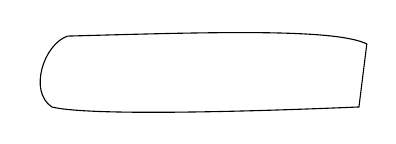
\begin{tikzpicture}[x=1cm,y=1cm]
\draw (0,0) .. controls (-.3,.2) and (-.1,.8) .. (.2,.9)
.. controls (2,.95) and (3.6,1) .. (4,.8)
--(3.9,0) .. controls (2,-.08) and (.4,-.1) .. (0,0);
\end{tikzpicture}}
\scanpage{50}
% archive foliation: 49
\hfill - 36 -\hfill n° 395

\deleted{
que $\|u_n\|<C$, $x_n=\sum_{k=1}^{n}\gamma(1-\gamma)^k u_k+(1-\gamma)^n e$ admette un inverse $t_n$, et $\|t_nz-t_{n-1}z\|<\dfrac{\delta}{2^n}$, $\|t_1z-z\|<\dfrac{\delta}{2}$. Posant $y_n=t_nz$, les $y_n$ tendent vers une limite $y\in A$, $x_n$ tend vers $x=\sum_{k=1}^{\infty}\gamma(1-\gamma)^{k-1}u_k$; x et y ont les propriétés requises).

23) a) Soient E un espace de Banach, $f:\mathbb{C}\longrightarrow E$ une fonction entière, et $\vartheta\longrightarrow p(\vartheta)=\sum_{\mu=k}^{m}c_\mu e^{\mu i\vartheta}$ un polynôme trigonométrique, $(c_k\ne0)$. On suppose que $|p(\vartheta)|\,\|f(re^{i\vartheta})\|\leq Mr^\alpha$ pour $r\geq r_0$, (M, $r_0$, $\alpha$ étant des constantes $\geq0$). Alors f est un polynôme de degré $\leq\alpha$. (Soient $f(\zeta)=\sum_{\nu=0}^{\infty}a_\nu\zeta^\nu$, et $J(r,p)=r^{-p}\int_0^{2\pi}p(\vartheta)f(re^{i\vartheta})e^{-(k+p)i\vartheta}\,d\vartheta$. On a $J(r,p)\longrightarrow0$ quand $r\longrightarrow+\infty$ si $p>\alpha$, et d'autre part $\lim J(r,p)=c_ka_p$).

b) Prouver de même que, si $\alpha$ est entier et si $r^{-\alpha}|p(\vartheta)|\,\|f(re^{i\vartheta})\|\longrightarrow0$ quand $r\longrightarrow+\infty$, f est un polynôme de degré $<\alpha$.

c) Soient A une algèbre de Banach \unsure{unipollente|unipotente}, x un élément quasi-nilpotent de A. On suppose que, pour un certain entier $n>0$, on a $r^{-n}|\cos^n\vartheta|\,\|(e-\lambda\unsure{z|x})^{-1}\|\longrightarrow0$ quand $r\longrightarrow+\infty$, $(\lambda=re^{i\vartheta})$. Alors $x^n=0$. (Utiliser b)).

\P\quad 24) a) Soient E un espace de Banach, $x:\mathbb{C}-\{1\}\longrightarrow E$ une fonction entière de $1/(\zeta-1)$, $x(\zeta)=\sum_{n=0}^{\infty}a_n\zeta^n$, $x(\zeta)=\sum_{n=0}^{\infty}b_n\zeta^{-n}$ les développements de x pour $|\zeta|<1$, $|\zeta|>1$ respectivement. On suppose $\|a_n\|=\unsure{o|O}(n^\alpha)$, $\|b_n\|=\unsure{o|O}(n^\alpha)$, $(\alpha>0)$. Alors $x(\zeta)$ est un polynôme en $1/(\zeta-1)$ de degré $<\alpha+1$. (Soit $\varepsilon>0$. On a $\|x(\zeta)\|\leq\varepsilon(1-r)^{-1-\alpha}$ pour $r_\varepsilon\leq r=|\zeta|<1$, $\|x(\zeta)\|\leq\varepsilon(1-r^{-1})^{-1-\alpha}$ pour $1<r<r'_\varepsilon$. Posant $1-\zeta=(\omega+\frac12)^{-1}$, $\omega=Re^{i\vartheta}$ montrer que, pour $0\leq r<1$ et $R\geq1$, on a $(1-r)^{-1}\leq\dfrac94\dfrac{R}{\cos\vartheta}$ et que, pour $1<r$ et $R\geq1$, $(1-r^{-1})^{-1}\leq\dfrac94\dfrac{R}{\cos\vartheta}$. Poser $y(\omega)=x(\zeta)$ et montrer que
}

\scanpage{51}
% archive foliation: 50
nienne sur le corps des fractions \deleted{de} L de K ?

On notera que même \unsure{dans|dams} le cas où $A=W(k)$, k alg. clos, le foncteur en question n'est pas \deleted{\unsure{essentiellem}} essentiellement surjectif.

Notons le

\uline{Problème} 5. \inserted{(A anneau de val. discrète complet d'inégales car.,k parf)} Expliciter le foncteur naturel qui va de la sous-catégorie pleine précédente de la catégorie des couples \deleted{d} $(M,\mathrm{Fil})$ d'un module de Dieudonné M sur \deleted{W} k (i.e. \deleted{sur} module sur W) et d'une filtration à deux crans de $M\otimes_W L$, vers les modules galoisiens sur L (\unsure{représent tions|représentations} \inserted{\unsure{vectoorielles|vectorielles} des dimension finie sur $\underline{Q}_p$ de} de $\mathrm{Gal}(\overline{L}/L)$)\deleted{dans des \unsure{repré} modules libres de type fini} Peut-on même définir ce foncteur \deleted{sur la sous-catégorie} de façon naturelle sans se borner à cette sous-catégorie pleine,en imposant seulement des conditions de rangs sur le gradué, mettons ?

\uline{Problème} 6. Revenant à un A comme dans Pb 4, peut-on trouver un foncteur \deleted{d'une} de la catégorie des couples $(M,\mathrm{Fil}^{1})$ d'un isocristal de Dieudonné \inserted{admissible} sur $A_{\unsure{o|0}}=A/pA$ (ou encore, sur $A_{\unsure{o|0}\,\mathrm{red}}\ \deleted{\unsure{\mathrm{perf}}}$) et d'une filtration en deux crans par modules localement libres de $(M_A)_p$, ayant le rang qu'il faut\deleted{\unsure{,}} (et soumis éventuellement à d'autres conditions ouvertes,\inserted{au sens Zar} assurant que le couple envisagé provient d'un isogroupe de BT sur A),vers les faisceaux p-adiques constants tordus sur $U=\mathrm{Spec}(A_p)$, qui exprime le foncteur du théorème (VII 10.8.2) précédent.

\deleted{4) Question des relations entre cohomologie cristalline et p-adique.}

\deleted{\deleted{Problème} \uline{Conjecture} 7. On peut, pour tout anneau de valuation discrète complet V d'inégales caractéristiques, de corps \deleted{des fractions} \unsure{rismduel|résiduel} parfait (pour simplifier), de corps des fractions L, trouver un foncteur canoniques sur une sous-catégorie pleine convenable des couples $(M,\mathrm{Fil}^{\deleted{\unsure{1}}})$ \deleted{\unsure{envisagé|envisagés}} dans le Pb 5 vers les}

\scanpage{52}
% archive foliation: 51
% Sheet read after 180-degree rotation.
\hfill - 35 -\hfill n° 393

\deleted{
21) Soient A une algèbre de Banach unipollente, $\Delta$ une partie ouverte de $\mathbb{C}$, $\lambda\longrightarrow R(\lambda)$ une application de $\Delta$ dans A telle que:
\[
(1)\qquad R(\lambda)-R(\mu)=-(\lambda-\mu)R(\lambda)R(\mu)
\]
quels que soient $\lambda$, $\mu\in\Delta$.

a) Soit $\lambda_0\in\Delta$. Pour tout $\lambda\in\Delta$ tel que $|\lambda-\lambda_0|\,\|R(\lambda)\|<1$, on a:
\[
R(\lambda)=\sum_{n=0}^{\infty}(\lambda_0-\lambda)^n R(\lambda_0)^{n+1}.
\]

b) Pour tout $\lambda\in\Delta$, $\dfrac{d^n}{d\lambda^n}R(\lambda)=(-1)^n n!\,R(\lambda)^{n+1}$.

c) Si R est holomorphe à l'infini, il existe z, j, $x\in A$ tels que $z^2=0$, $j^2=j$, $zj=jz=0$, $x\in jAj$, et $R(\lambda)=z+jR(\lambda,x)$ pour $|\lambda|$ assez grand. (Ecrire $R(\lambda)=\sum_{n=0}^{\infty}c_n\lambda^{-n}$ pour $|\lambda|>\lambda_0$, et exprimer que R satisfait à (1). On peut poser $c_0=z$, $c_1=j$, $c_2=x$).

d) Pour que R soit la résolvante d'un élément de A, il faut et il suffit que $R(\lambda_0)$ soit inversible pour un $\lambda_0\in\Delta$.

e) Pour tout $x\in A$, la fonction $\lambda\longrightarrow\sum_{n=0}^{\infty}(\lambda_0-\lambda)^n x^{n+1}$ satisfait à (1) pour $|\lambda-\lambda_0|\,\|x\|<1$.

\P\quad 22) a) Soient B une algèbre de Banach unipollente, $w\in B$, $C>1$ et $\varepsilon>0$. Il existe $\eta>0$ tel que les conditions $u\in B$, $\|u\|<C$, $\|uw-w\|<\eta$, $0\leq\gamma\leq1/4C$ impliquent $\|yw-u\|<\varepsilon$, où $y=[(1-\gamma)e+\gamma u]^{-1}$.

b) Soit A une algèbre de Banach. On suppose qu'il existe une constante C telle que, pour tout $\varepsilon>0$ et tous $x_1,....,x_n\in A$, il existe $u\in A$ avec $\|u\|<C$, $\|ux_1-x_1\|<\varepsilon,....,\|ux_n-x_n\|<\varepsilon$. Pour tout $z\in A$, il existe $x,y\in A$ tels que $z=xy$, $y\in\overline{Az}$, $\|z-y\|<\delta$. (On peut supposer $C>1$. Soit $\gamma=1/4C$. Appliquant a) dans $\widetilde{A}$, déterminer par récurrence une suite $u_1,u_2,....$ dans A telle
}

\scanpage{53}
% archive foliation: 52
\[
\begin{array}{l}
\left\{\begin{array}{l}
\displaystyle\sum_1^i\lambda'_j\leq\displaystyle\sum_1^i\lambda_j\\
\displaystyle\sum_{\unsure{1}}^{\unsure{n}}\lambda'_j=\displaystyle\sum\lambda_j
\end{array}\right.\\
\qquad\unsure{\Vert}\\
\qquad\displaystyle\sum i\unsure{h'_i}
\end{array}
\]
\margin{\unsure{mult de} pentes de Hodge}
\figure{\begin{tikzpicture}\draw (0,0)--(3,.9) .. controls (3.2,1) and (3.1,1.1) .. (3.05,1.1);\end{tikzpicture}}
\hrule

\margin{\unsure{Sur un th de Tate.}}
\uline{Sur un théorème de Tate.} (Devrait venir avec foncteur mystérieux !)

C'est le théorème suivant (Driebergen ....):

\uline{Th.} (Tate): Soit S un schéma noethérien normal intègre dont le corps des fonctions \inserted{$k(\eta)$} est de car. zero, Alors le foncteur
\[
\mathrm{BT}(S)\longrightarrow\mathrm{BT}(\eta)
\]
est pleinement fidèle.

Ainsi, un groupe de BT sur S est connu \inserted{à isom unique près} quand on connaît la représentation p-adique qu'\deleted{elle}\inserted{\unsure{il}} définit de $\pi_1(\eta)=\mathrm{Gal}(\overline{k(\eta)}/k(\eta))$. Prenant d'abord le cas où S est le spectre d'un anneau de valuation discrète complet V d'inégales car. , de corps \deleted{des} résiduel k parfait, la question se pose donc

a) De caractériser les modules galoisiens qu'on peut obtenir (Tate donne des conditions nécessaires: les modules en question doivent être du type de ``Hodge-Tate'' );

b) De trouver un foncteur ``explicite'' sur la catégorie de ces modules galoisiens, vers les F-cristaux sur k M muni d'une filtration de $M\otimes_W\unsure{W|V}$.

\margin{\uline{Problème}}
Le théorème de Tate suggère de plus que le ``foncteur mystérieux'' qui va des F-cristaux sur k filtrés sur L, vers les $\underline{Q}_p$-modules galoisiens sur L, est pleinement fidèle, et qu'on doit pouvoir donc \deleted{définir un \unsure{foncteu|foncteur}} expliciter un foncteur quasi-inverse (non moins mystérieux), allant d'une sous-catégorie pleine convenable des $\underline{Q}_p$-modules galoisiens sur L (sans doute contenue dans celle des modules galoisiens du type de Hodge-Tate) vers les F-cristaux sur k filtrés sur L.

D'autre part, on conjecture que dans le th. de Tate ci-dessus, la restriction au cas où $\deleted{k}\inserted{k(\eta)=L}$ est de car. nulle est inutile, Le seul cas qui offre

\scanpage{54}
% archive foliation: 53
un Pb. est celui où $k(\eta)=L$ est de car.p (cas d'égales caractéristiques). On peut alors penser à attaquer le Pb via la théorie de Dieudonné (supposant résolu le Pb 1) et via le

\uline{Problème} n° ... Soit S un schéma noethérien normal \deleted{de car} intègre de car. p, de point générique $\eta$. Est-il vrai que le foncteur de restriction
\[
\mathrm{Cris\ loc\ lib}\ (S)\longrightarrow\mathrm{Cris\ loc\ lib}\ (\eta)
\]
(ou du moins le foncteur analogue pour F-cristaux) est pleinement fidèle ?

On est ramené facilement au cas où S est le spectre d'un anneau de la forme $\unsure{k[(t)]|k[[t]]}$, avec k alg. clos, auquel cas l'énoncé s'explicite en termes de Modules avec connexions formelles .... Il semble que si la réponse au Pb précédent est affirmative, \deleted{ainsi que} et si on sait faire la théorie de \unsure{Dieudonnén|Dieudonné} sur un anneau \uline{parfait} (avec \uline{équivalence} de catégories alors on aura démonstration du th. de Tate en égales car.

\scanpage{55}
% archive foliation: 54

$\chi$ et $\chi_!$

\scanpage{56}
% archive foliation: 55

$k$ corps

\diagram{\begin{array}{lll}
\mathcal{E}_{\chi!}&\text{espaces topologiques }\inserted{\text{loc. comp.}\unsure{\text{ts}}}\text{ tels que }H^*_!(\unsure{X},k)&\text{de dim finie sur }k\\
\mathcal{E}_{\chi}&\rule{7cm}{0.4pt}\quad H^*(X,k)&\rule{4cm}{0.4pt}
\end{array}}
\margin{coh. \deleted{\unsure{faisceautique}} \inserted{singulière}}
\margin{coh. singulière}

\textcircled{a} \deleted{$\unsure{\chi(X)=\chi_!(X)}$} Si $X$ compact, $X\in\mathcal{E}_{\chi!}\Longleftrightarrow X\in\mathcal{E}_{\chi}$, et alors
\[
\chi_!(X)=\chi(X).
\]
\margin{trivial}

\textcircled{b} Si $Y$ fermé dans $X$ \inserted{loc. cpt}, alors si deux des espaces $X,Y,X-Y$ sont dans $\mathcal{E}_{\chi!}$, le troisième aussi, et on a
\[
\chi_!(X)=\chi_!(Y)+\chi_!(X-Y)
\]
(résulte de suite ex. de cohomologie à supp. cpts)

\textcircled{c} Si $X',X''$\deleted{$\unsure{X}$} fermés dans $X$ de réunion $X$, alors si trois parmi les quatre \unsure{espaces|esp.} $X,X',X'',X'\cap X''$ sont dans $\mathcal{E}_{\chi}$, le quatrième aussi, et on a
\[
\chi(X)=\chi(X')+\chi(X'')-\chi(X'\cap X'')
\]
(résulte de suite ex. de Mayer-Vietoris

\deleted{\textcircled{d}}
\[
[\text{Même}\quad X,X'\cap X''\in\mathcal{E}_{\chi}\Longrightarrow X',X''\in\mathcal{E}_{\chi}]
\]

\textcircled{d} Si $X$ \deleted{\unsure{est rétracte de}} \inserted{dominé} homotopiquement par $X'$
(\diagram{\begin{tikzcd}[column sep=large]
X \arrow[r, shift left, "i"] & X' \arrow[l, shift left, "j"]
\end{tikzcd}}
$\qquad ji\unsure{\simeq|\sim}\mathrm{id}_X\quad$) alors $X'\in\mathcal{E}_{\chi}\Longrightarrow X\in\mathcal{E}_{\chi}$, d'où
\[
(X\sim X')\unsure{\Longleftrightarrow|\Longrightarrow}(X\in\mathcal{E}_{\chi}\unsure{\Longrightarrow|\Longleftrightarrow}X'\in\mathcal{E}_{\chi}),
\]
et de plus on a alors
\[
\chi(X)=\chi(X')
\]

\textcircled{e} \deleted{\unsure{Si} $X$ \unsure{se contracte à un pt,}} $\operatorname{Card}X\leq1\Longrightarrow X\in\mathcal{E}_{\chi}$, de plus on a
\[
\chi(pt)=1
\]
(de plus $\chi(\varnothing)=0$, grâce à \unsure{e)|c)} p.ex) \margin{(trivial)}

\scanpage{57}
% archive foliation: 56
% Sheet read after rotation through 180 degrees.

10.

5.2. \uline{Evaluation de la politique de recherche des établissements}

La D.E.S.U.R. ne sera crédible auprès de la D.G.R.S.T. et par conséquent n'obtiendra des crédits suffisants que si elle est capable de porter un jugement sur la valeur des résultats de recherche de chaque établissement et sur la façon dont les établissements conduisent leur politique de recherche. Actuellement les services de la D.E.S.U.R. disposent de nombreuses données sur les établissements :

\begin{itemize}
\item[-] le nombre des thèses soutenues
\item[-] le nombre et la qualité des publications
\item[-] le nombre d'associations avec les autres établissements de recherche
\item[-] le nombre des contrats
\item[-] évolution de la carrière du personnel
\end{itemize}

Le danger est grand de voir s'instituer un système purement numérique, alimenté par ces critères, et fournissant, par un ordinateur, \unsure{le:montant|le montant} des crédits de l'université. Juger la recherche conduite par un établissement est une opération délicate ; il est donc envisagé de placer, auprès du directeur des enseignements supérieurs et de la recherche un groupe de personnalités indépendantes capables de faire la synthèse des renseignements recueillis sur un établissement pour porter un jugement global qui restera confidentiel.

5.3. \uline{La responsabilité de la D.E.S.U.R.}

Les deux branches du Secrétariat d'Etat qui supportent la recherche dans les établissements d'enseignement supérieur, la D.E.S.U.R. et le C.N.R.S. doivent pratiquer une politique différente , quoique étroitement complémentaire. Le C.N.R.S. est une entreprise de recherche centralisée, qui agit par discipline ; il aide, dans un tel établissement tel laboratoire parce que cela est utile au programme de recherche. La D.E.S.U.R. agit par établissement ; elle aide chaque établissement à développer le programme qu'il propose, sous réserve qu'il contribue à l'une des missions spécifiques de la recherche universitaire.

Cela suppose la mise au point d'une politique de répartition des moyens complémentaires (\S\ 4.2.) qui en s'ajoutant aux moyens de base (\S4.1.) conditionnent la politique de recherche de l'établissement.

.../...

\scanpage{58}
% archive foliation: 57

\uline{Conclusions provisoires} (on pose $\overline{\mathbb{R}}=[-\infty,+\infty]$

\margin{\textcircled{1} On a $X',X''\in\mathcal{E}_{\chi}$ (resp. $\mathcal{E}_{\chi!}$) $\Longleftrightarrow X'\amalg X''\in\mathcal{E}_{\chi}$ (resp. $\mathcal{E}_{\chi!}$), et alors
\deleted{\unsure{résulte de c et e}}
\[
\chi(X)=\chi(X')+\chi(X'')\quad(\text{resp.}\ldots)
\]
résulte de c) et e) $(\varnothing\in\mathcal{E}_{\chi})$ resp. de b)}

\textcircled{\unsure{2}} \deleted{$\unsure{n\geq1}$}\inserted{$\forall n\in\mathbb{N}$}, $R^n,\overline{R}^n,B^n,S^n\in\mathcal{E}_{\chi}\cap\mathcal{E}_{\chi!}$, de plus
\[
\left\{\begin{aligned}
\chi(\unsure{R^n})&=\chi(\overline{R}^n)=\chi(B^n)=1\\
&\overset{\text{''}}{\chi_!}(\overline{R}^n)=\overset{\text{''}}{\chi_!}(B^n)\\
\chi_!(R^n)&=(-1)^n
\end{aligned}\right.
\qquad
\chi(S^n)=\chi_!(S^n)=1+(-1)^n
\]

\uline{Dém} $R^n,\overline{R}^n,B^n\sim pt$, donc par d) et e) ils sont $\in\mathcal{E}_{\chi}$ ; comme $\overline{R}^n,B^n$ compacts, par b) ils sont aussi $\in\mathcal{E}_{\chi!}$.

On a $S^n=S^n_+\cup S^n_-$ et $S^n_+\cap S^n_-\simeq S^{n-1}$, \inserted{Or $S^n_+\simeq S^n_-\simeq B^n$ donc $\in\mathcal{E}_{\chi}$} donc on conclut de c) par réc. sur $n$ que $S^n\in\mathcal{E}_{\chi}$ (\uline{NB} $S^0=\{pt\}\amalg\{pt\}\in\mathcal{E}_{\chi}$ par \unsure{d)|1)} et e), et $\chi(S^0)=1+1=2$), et on trouve
\[
\chi(S^n)=\chi(S^n_+)+\chi(S^n_-)-\chi(S^{n-1})\unsure{\ne|=}2-\chi(S^{n-1}),
\]
d'où par récurrence sur $n$ $\chi(S^n)=1+(-1)^n$. Comme $S^n$ cpt, $S^n\in\mathcal{E}_{\chi!}$, et $\chi_!(S^n)=\chi(S^n)$ par (a). Enfin, $R^n\simeq S^n-pt$, donc par (b) $R^n\in\mathcal{E}_{\chi!}$ et
\[
\chi(R^n)=\chi(S^n)-\chi(pt)=(1+(-1)^n)-1=(-1)^n,
\]
cqfd.

\textcircled{3} Soit $X_{-1}=\varnothing\unsure{\subset}X_0\subset X_1\subset\cdots\subset X_n=X$ filtration de l'espace $X$, tel que $\forall\,0\leq i\leq n$, $X_i-X_{i-1}$ \deleted{\unsure{est} $\unsure{\mathbb{R}}$} a un nb fini $f_i$ de comp. connexes ttes homéom. à $\mathbb{R}^i$ (i.e. $X_i-X_{i-1}\simeq f_i\times\mathbb{R}^i$). Alors $X\in\mathcal{E}_{\chi!}$, et on a
\[
\chi_!(X)=\sum(-1)^i f_i
\]
(donc si $X$ est cpt, on a $X\in\mathcal{E}_{\chi}$ et $\chi(X)=\sum(-1)^i f_i$ ...

\figure{\begin{tikzpicture}[x=1cm,y=1cm]
\draw (0,2)--(0,1.2)--(1.4,1)--(2.2,-.2)--(3.3,-.2);
\draw (0,1.5)--(3.4,1.5);
\end{tikzpicture}}
\scanpage{59}
% archive foliation: 58
% Sheet read after rotation through 180 degrees.

9.

4.3. - \uline{La politique de recherche des établissements}

Un établissement d'enseignement supérieur possède en général un Conseil scientifique. Il lui revient de définir les grandes lignes de la politique scientifique de l'établissement. L'objectif est clair :

\begin{itemize}
\item[-] compte tenu des moyens en bâtiments, personnel enseignant et technicien, comment utiliser les crédits spécifiques pour la recherche de façon optimum, pour faire la meilleure recherche, \unsure{celle} qui assure le renon de l'établissement et lui permet de s'associer avec les grands établissements de recherche, en premier lieu avec le C.N.R.S.
\item[-] Il appartient au Conseil scientifique de conduire la politique de recherche de l'établissement, sous la responsabilité du Président. La recherche est l'affaire de l'ETABLISSEMENT, chacun étant solidaire pour la mener à bien.
\end{itemize}

Une politique recherche est, typiquement, celle que fait naitre des équipes qui deviennent peu à peu des équipes associées avec le C.N.R.S. et avec l'I.N.S.E.R.M.. La collaboration prolongée de l'établissement à frais partagés avec un organisme de recherche est le critère de réussite d'une politique de recherche.

5 - \uline{La politique ``recherche'' de la D.E.S.U.R.}

5.1. \uline{La D.E.S.U.R. doit remplir une mission de complexe dans le cadre du plan-recherche lui permettant} :

a) d'agir ``en aval'' au niveau des établissements en respectant leur autonomie ; elle ne peut donner des ordres ni définir des programmes \uline{a priori} ; elle doit par contre, effectuer un contrôle a postériori, pour avoir des éléments de jugement sur l'activité de recherche des établissements.

b) d'agir ``en amont'' au niveau national en tenant sa place, parmi une dizaine d'organismes fortement hiérarchisés, pour obtenir sa part de l'enveloppe-recherche. La D.E.S.U.R. doit être ``crédible'' par la D.G.R.S.T.

\scanpage{60}
% archive foliation: 59

\textcircled{f}
\[
\begin{aligned}
X,Y\in\mathcal{E}_{\chi!}&\Longrightarrow X\times Y\in\mathcal{E}_{\chi!}\quad\text{et on a}\quad\chi_!(X\times Y)=\chi_!(X)\chi_!(Y)\\
X,Y\in\mathcal{E}_{\chi}&\Longrightarrow X\times Y\in\mathcal{E}_{\chi}\quad\text{et on a}\quad\chi(X\times Y)=\chi(X)\chi(Y).
\end{aligned}
\]
(La première assertion résulte de Künneth pour $H^*_!(X\times Y,k)$, la deuxième de Künneth pour $H_*(X\times Y,k)$, dont le dual est $H^*(X\times Y,k)$, donc qui permet de tester l'appartenance à $\mathcal{E}_{\chi}$ et la valeur de $\chi$ ...)

\textcircled{g} Soit $f:X\unsure{-|\longrightarrow}Y$ fibration loc. triviale de fibre $F$.

Si $Y,F\in\mathcal{E}_{\chi!}$, alors $X\in\mathcal{E}_{\chi!}$, et on a
\[
\chi_!(X)=\chi_!(Y)\chi_!(F).
\]
Énoncé analogue pour \inserted{$Y,F\in$}$\mathcal{E}_{\chi}$ et \deleted{$\unsure{\chi(X)=}$}
\[
\chi(X)=\chi(Y)\chi(F)
\]
\margin{\unsure{cum|avec} \unsure{léger} grain de sel}
\figure{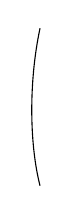
\begin{tikzpicture}[x=1cm,y=1cm]\draw (0.15,2) .. controls (0,1.3) and (0.02,0.5) .. (0.15,0);\end{tikzpicture}}

\uline{Dém}. On a
\[
H^*_!(X)\Longleftarrow E_2^{pq}=H^p_!\left(Y,\underbrace{R^q f_!(\unsure{k_X})}_{\substack{\text{syst. local sur }Y\\\text{à fibres }\sim H^q_!(F)}}\right)
\]
donc \uline{sous réserve} qu'on sache que $E_2^{\unsure{**|pq}}$ de dim finie, on trouve $X\in\mathcal{E}_{\chi}$ et
\[
\begin{aligned}
\chi(X)&=\sum_{pq}(-1)^{p+q}\operatorname{rg}_k H^p_!(Y,R^q f_!(k_X))\\
&=\sum_q(-1)^q\underbrace{\sum_p(-1)^p\operatorname{rg}_k H^p_!(Y,R^q f_!(k_X))}_{b^q_!(F)\chi_!(Y)}\\
&=\chi_!(Y)\deleted{\unsure{\chi}}\sum_q(\unsure{+1|-1})^q b^q_!(F)=\chi_!(Y)\chi_!(F)
\end{aligned}
\]

Il faut prouver

\figure{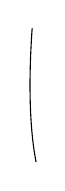
\begin{tikzpicture}[x=1cm,y=1cm]\draw (0.03,1.7) .. controls (-0.02,1) and (0,0.4) .. (0.08,0);\end{tikzpicture}}
\uline{Lemme} Soit $\mathcal{R}$ syst. local de $k$-vectoriels sur \deleted{\unsure{$X$ loc cpt,}} $Y\in\mathcal{E}_{\chi!}$, à fibres de rang \inserted{fini} $b$. Alors
\[
\chi_!(Y,\mathcal{R})\overset{\mathrm{déf}}=\sum_p(-1)^p H^p(Y,\mathcal{R})
\]
existe (i.e. $\unsure{\sum|\bigoplus}_p H^p(Y,\mathcal{R})$ de dim finie sur $k$) et on a
\[
\chi_!(Y,\mathcal{R})=b\chi_!(Y).
\]
\margin{\textcircled{\unsure{gn}}}

Marche tout au moins si $Y$ \deleted{triangulable} \inserted{admet filtration finie} avec $Y_i-Y_{i-1}$ somme finie de cellules \inserted{$Z_{ij}$}$\simeq R^{\delta_{ij}}$, car

On a :
\[
\begin{aligned}
\chi_!(Y,\mathcal{R})&=\sum_{ij}\chi_!(Z_{ij},\mathcal{R})=\sum_{ij}b\chi_!(Z_{ij})\\
&=b\sum\chi_!(Z_{ij})=b\chi_!(Y).
\end{aligned}
\]
\margin{(\unsure{ct.} sur $Z_{ij}$\unsure{)|]}}

\scanpage{61}
% archive foliation: 60
% Sheet read after rotation through 180 degrees.

8.

\diagram{\begin{array}{@{\vdots\;}l@{\;\vdots\;}r@{\;\vdots\;}r@{\;\vdots\;}r@{\;\vdots\;}r@{\;\vdots\;}r@{\;\vdots\;}r}
\hline
&1971&1972&1973&1974&1975&1976\\\hline
\begin{array}{l}\text{Fonctionnement}\\\text{(MF) Chap. 36.15}\end{array}&190&206&223&249&257&275\\\hline
\begin{array}{l}\text{Equipement (MF)}\\\text{Chap. 56-10 (50)}\end{array}&87&92&93&93&104&79\\\hline
\text{TOTAL}&277&298&316&342&361&3\deleted{\unsure{9|5}}\inserted{5}4\\\hline
\end{array}}

La quasi totalité du crédit de fonctionnement est réparti en tenant compte de critères quantitatifs :
\begin{itemize}
\item[-] nombre d'enseignant chercheurs de l'établissement
\item[-] nombre de thèses soutenues
\item[-] nombre d'association réalisées avec d'autres établissements de recherche
\item[-] investissements réalisés au cours des six dernières années au profit des formations de recherche.
\item[-] nouvelles actions originales de l'établissement.
\end{itemize}

Cette répartition est effectuée avant le début de l'année civile. La totalité du budget 1976 est donc actuellement répartie.

Le budget d'équipement est réparti par la D.E.S.U.R. sous la forme de deux grandes masses :

\begin{itemize}
\item[-] des constructions spécifiques pour la recherche, et des investissements de matériels de grande importance (ordinateurs, matériels communs à plusieurs établissements) ; ces opérations sont pilotés par la DESUR en accord avec les établissements.
\item[-] du matériel ``moyen'' pour la recherche, ces appareils sont attribués à l'établissement sur sa proposition, après examen et approbation par les experts de la DESUR.
\end{itemize}

\scanpage{62}
% archive foliation: 61

\margin{$(\unsure{g_2|g'_2})$}
Cela marche aussi si \deleted{$\unsure{\mathcal E|X}$} $Y$ \inserted{cpt} admet des $\mathrm{rec.}^{\mathrm{ts}}$ arbitrairement fins \inserted{finis} par des $Y_i$ \inserted{fermés ou ouverts} tels que les intersections
$Y_{i_1}\cap Y_{i_2}\cap\cdots\cap Y_{i_\nu}$ $(\nu\ge1)$ de tels $Y_i$ soient $\in\mathcal{E}_{\chi!}$ ....

Dans le cas de $\chi$, on utilise la suite spectrale d'\uline{homologie}, on est ramené à :

\uline{Lemme} Soit $\mathcal R$ syst. local de $k$-vectoriels sur $Y\in\mathcal E_\chi$, fibres de rang \inserted{fini} $b$. Alors
% Two short vertical grouping strokes stand at the left of this lemma.
\figure{\begin{tikzpicture}\draw (0,0)--(0,.65);\draw (0,-.45)--(0,-.2);\end{tikzpicture}}
\[
\chi(Y,\mathcal R)\overset{\mathrm{déf}}=\sum_p(-1)^p
\underbrace{H_{\inserted{p}}^{\deleted{\unsure{p}}}(Y,\mathcal R)}_{\text{le dual est }H^p(Y,\check{\mathcal R})}
\]
existe et :
\[
\chi(Y,\mathcal R)=b\chi(Y).
\]
Cela marche pourvu qu'on fasse l'hyp. \deleted{\unsure{que}} \inserted{\unsure{que}} $Y$ est $\sim Y'$ satisfaisant la condition $(\unsure{g_2|g'_2})$.

\figure{\begin{tikzpicture}\draw (0,0)--(.65,0);\draw (.15,.08)--(.52,.08);\end{tikzpicture}}

\deleted{\unsure{On va se borner}}

\textcircled{h} Définissons $\mathcal C_{-1}=$ \unsure{Ens.|cls.} réduit \unsure{:|à} l'espace vide
et si $n\ge0$ $\mathcal C_n^{\deleted{\unsure{\mathrm{loc}|\mathrm{cpt}}}}=$ \deleted{catégorie} \inserted{classe} des espaces cpts \inserted{$X$} tels que tt pt \inserted{$x\in X$} ait un voisinage $C_x$ tel qu'il existe un espace compact $S\in\unsure{\mathcal E|\mathcal C}_{n-1}$ et un homéom. $\operatorname{Cône}(S)\simeq C_x$ transformant le sommet du cône en $x$.

\[
\mathcal C_\infty=\bigcup_n\mathcal C_n\qquad\text{(espaces loc. côniques)}
\]
\[
\mathcal E_\infty=\deleted{\text{esp}}\text{ des espaces loc. cpts }\inserted{\text{séparés}}X\text{ tels que }\widehat X
\]
soit loc. cônique i.e. $\in C_\infty$.

\margin{\uline{NB}
$\mathcal E_0$ espaces discrets

$\mathcal E_1$ 1-complexes topologiques

$\mathcal E_2$ espaces loc. triangulables de dim $\le2$ [ils sont triangulables dans le cas cpt]

$\mathcal E_3$ espaces loc. triangulables de dim $\le3$ \deleted{[\unsure{ils sont triang. dans} le cas cpt]}

$\mathcal E_4$ esp. loc.\,$\cdots$\,dim $\le4$ (Moïse)

S'ils sont cpts, il n'est pas clair qu'ils sont triangulables ....}
% Right grouping brace beside the first marginal list; angular bracket beside its continuation.
\figure{\begin{tikzpicture}\draw (0,1)..controls(.15,.9)and(.02,.75)..(.18,.6)..controls(.02,.45)and(.15,.2)..(0,0);\draw (.25,0)--(.42,0)--(.42,-.7)--(.25,-.7);\end{tikzpicture}}

\uline{Prop} $\unsure{\mathcal C|\mathcal E}_\infty\subset\mathcal E_\chi\cap\mathcal E_{\chi!}$

Soit $X\in\mathcal E_\infty$. Si $X$ est cpt, \inserted{donc $X\in C_\infty$} comme $X$ est loc. contractile,
on sait que \deleted{\unsure{$X\in$}}$\mathcal E_\chi$, donc $X\in\mathcal E_{\chi!}$. \unsure{Cas|Car} \deleted{\unsure{$X$ général}} \inserted{\unsure{général}} : $X$ loc.
cpt $=\widehat X-(\unsure{\omega|\infty})$, avec $\widehat X\in\mathcal E_\infty$, on a $\widehat X\in\mathcal E_{\chi!}$, donc
$\widehat X-\unsure{\omega|\infty}=X\in\mathcal E_{\chi!}$ par (b). Pour prouver $X\in\mathcal E_\chi$, prenons un
$C_x\simeq C(S)$, prenons un homothétique $\frac12 C_x=T$, et

\scanpage{63}
% archive foliation: 62; reused typescript, upside down in scan.

\unsure{1.|7.}

- considération la demande des besoins locaux.

4 - \uline{Comment faire de la recherche dans un établissement d'enseignement supérieur}

4.1. \uline{Les établissements et leurs moyens de base} :

Un établissement d'enseignement supérieur possède du personnel enseignant dont une partie seulement de l'activité est consacrée à l'enseignement ; le reste peut donc être consacré à la recherche. Il est difficile d'avancer une estimation chiffrée de ce partage, qui varie selon les disciplines. Considérons en première approximation que le temps consacré à l'activité de recherche est de 40\% en moyenne du temps de l'enseignant chercheur. Par ailleurs, l'établissement dispose de locaux construits et entretenus à l'aide de crédits inscrits sur des chapitres budgétaires de la D.E.S.U.R. (non inclus dans l'enveloppe recherche) Enfin, l'établissement dispose de personnel administratif, technique, ouvrier et de service (A.T.O.S.) dont une part de l'activité est consacrée à la recherche. Il apparait donc d'emblée que chaque établissement possède un potentiel ``hors enveloppe-recherche'', qu'il doit mobiliser pour le consacrer à la recherche.

Pour chiffrer ce budget, hors enveloppe-recherche, qui est pourtant consacré à la recherche, on pourrait prendre 40\% de la masse salariale des enseignants et admettre, en première approximation, que 30\% du personnel A.T.O.S. effectue un travail de recherche. En admettant en outre qu'une part du budget général du secrétariat d'Etat (chapitre 36-11) contribue à la recherche (ne serait-ce que par le paiement des dépenses de chauffage des bâtiments ...), on arrive en 1975 à une approximation des dépenses pour la recherche de l'ordre de 1 100 à 1 200 millions de francs. Il peut donc être constaté que par le simple fait qu'elle rétribue à plein temps du personnel qui fait de l'enseignement à temps partiel, l'ensemble des établissements de la D.E.S.U.R. apporte au budget ``recherche'' une somme supérieure au milliard de francs.

4.2. \uline{Les crédits de la D.E.S.U.R. pour constituer ces moyens}

La D.E.S.U.R. dispose de deux chapitres budgétaires,d'un de ``fonctionnement'', l'autre ``d'équipement'', qui permettent d'aider cet effort de recherche dans chaque établissement. Le tableau ci-après indique l'évolution de ces budgets (millions de francs courants)

\scanpage{64}
% archive foliation: 63

Soit $X'=\widehat X-\mathring T$, qui est cpt. \deleted{et $\in\unsure{\mathcal C|\mathcal E}$}. On vérifie

\margin{\uline{vérifier}}

a) $X'\in C_\infty$ donc $X'\in\mathcal E_\chi$

b) $X'\sim X=\widehat X-\omega$ donc $X\in\unsure{\mathcal E_{\chi!}|\mathcal E_\chi}$.

\uline{NB} On trouve
\[
\chi(X)=\chi(\widehat X-\mathring T)=\chi(\widehat X)-\underbrace{\chi(T)}_{\substack{\unsure{\Vert|=}\\\unsure{1}}}+\chi(\partial T)
\]
et $\chi(T)=1$ car $T$ contractile, donc
\[
\chi(X)=\chi(\widehat X)-1+\chi(\underbrace{\partial T}_{\substack{\Vert\\S_\omega}})=\chi_!(X)+\chi(\partial T)\qquad\text{i.e.}
\]
\diagram{\boxed{\begin{array}{ll}
\chi(X)-\chi_!(X)=\chi(S_\omega)&\\
&\searrow\ \begin{array}{l}\text{exprime la ``structure}\\\text{locale de }X\text{ à l'infini''}\end{array}
\end{array}}}

\scanpage{65}
% archive foliation: 64; reused typescript, upside down in scan.

\begin{flushright}6.\end{flushright}

3.3. \uline{Les objectifs de recherche spécifiques des établissements d'enseignement supérieur.}

3.3.1. \uline{Mémorisation et diffusion de la connaissance} :

- rassemblement de la connaissance ; conservation de la connaissance ; mise en forme et diffusion de la connaissance. Cette diffusion ne sera pas limitée aux seuls étudiants à plein temps mais étendue vers toute personne intéressée et produite par tous supports(articles, ouvrages, collections, expositions) et toutes prestations (aide technique à l'industrie, études ...). La recherche pédagogique entre dans ce cadre.

3.3.2. \uline{Contribution à l'accroissement de la connaissance}

- en collaborant avec d'autres établissements de recherche, dans le cadre d'associations : l'établissement d'enseignement supérieur apporte une part des moyens, et une part importante du personnel compétent.

- en maintenant un état de ``fermentation intellectuelle'' permettant de faire naître des nouveaux domaines de recherche, notamment par le contact entre les diverses disciplines\unsure{.|;} Les nouvelles idées de recherche\inserted{,} initiées par l'établissement\inserted{,} doivent\inserted{,} ensuite être développées dans le cadre d'associations.

3.3.3. \uline{Formation par la recherche des futurs cadres de la nation.}

- Ceci exige un couplage de l'établissement avec des formations de recherche, où les étudiants en fin d'études pourront aller s'initier à la recherche en préparant une thèse de spécialité. La formation initiale et permanente des enseignants des établissements d'enseignement supérieur entre dans ce cadre. -

3.3.4. \uline{Contribution à l'animation intellectuelle et socio-économique de la région} :

- Les universités sont en effet les seuls établissements à vocation de recherche qui n'ont pas leur siège à Paris, et dont le programme n'est pas commandé par l'autorité centrale. Elles doivent plus que jamais s'ouvrir aux préoccupations de leur région en prenant en

\scanpage{66}
% archive foliation: 65

\uline{Th} Sur la cat. $\mathcal E_\infty$ des espaces loc. cpts séparés et \deleted{\unsure{cônes}} ``loc. côniques partout'' (y compris à l'$\infty$), on peut trouver deux fonctions numériques \inserted{$\chi_!,\chi$} (à valeurs $\in\mathbb Z$) satisfaisant les conditions (où tous les espaces écrits sont supposés $\in\mathcal E_\infty$)

\textcircled{a} $\chi_!(X)=\chi(X)$ si $X$ cpt

\textcircled{b} $Y$ fermé dans $X$ $\Longrightarrow\quad\chi_!(X)=\chi_!(Y)+\chi_!(\unsure{Y|X}-Y)$

\textcircled{c} $X',X''$ fermés dans $X$ $\Longrightarrow\quad\chi(X)=\chi(X')+\chi(X'')-\chi(X'\cap X'')$

\textcircled{d}
\[
\left\{\begin{aligned}
X\sim X'&\Longrightarrow\chi(X)=\chi(X')\\
X\simeq X'&\longrightarrow\chi_!(X)=\chi_!(X')
\end{aligned}\right.
\]

\textcircled{e} $\chi(\mathrm{pt})=1$

\textcircled{f}
\[
\begin{aligned}
\chi_!(X\times Y)&=\chi_!(X)\chi_!(Y)\\
\chi_{\deleted{\unsure{!}}}(X\times Y)&=\chi(X)\chi(Y)
\end{aligned}
\]

\textcircled{g} Si $f:X\longrightarrow Y$ fibration loc triviale de fibre $F$,
\[
\left\{\begin{aligned}
\chi_!(X)&=\chi_!(Y)\chi_!(F)\\
\chi(X)&=\chi(Y)\chi(F)
\end{aligned}\right.
\]
tout au moins si $Y$ est un polyèdre relatif (diff. de deux polyèdres, l'un plongé dans l'autre linéairement...)
\margin{j'ignore si c'est vrai sans telle restriction}
\figure{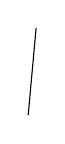
\begin{tikzpicture}\draw (0.1,1.1)--(0,0);\end{tikzpicture}}

Si \deleted{\unsure{le}} $X\in\mathcal E_\infty$ de sorte que $\widehat X\in\mathcal E_\infty$, on a

\textcircled{h}
\[
\left\{\begin{aligned}
\chi_!(X)&=\chi(\widehat X)-1\\
\chi(X)-\chi_!(X)&=\chi(S)\qquad\text{où }S\text{ est le ``}\unsure{\text{frontière}|\text{frontier}}\text{ à l'infini'' de }X.
\end{aligned}\right.
\]

Enfin, \unsure{les restrictions|la restriction} de \deleted{$\unsure{\chi|\mathcal E}$} $\chi$ et $\chi_!$ aux polyèdres relatifs sont uniquement déterminées par les propriétés \textcircled{a} à \textcircled{e}, et on a \deleted{\unsure{le}}, si $X$ muni d'une filtration cellulaire
\[
\chi_!(X)=\sum(-1)^i\unsure{\widehat f_i|f_i}\qquad\text{(formule d'Euler)}
\]
\margin{j'ignore si $\chi$ et $\chi_!$ sont caractérisés par a) à e) sur tout $\mathcal E_\infty$}
\figure{\begin{tikzpicture}\draw (0,1.8) .. controls (-0.1,1.2) and (0.1,0.6) .. (0.25,0);\end{tikzpicture}}

\scanpage{67}
% archive foliation: 66; reused typescript, upside down in scan.

\begin{flushright}5.\end{flushright}

3.2. \uline{Les missions d'enseignement et les missions de recherche}

- Les établissements ont-ils des missions de recherche ? C'est là une question à nous poser et à laquelle il importe de répondre en allant au fond du problème.

En effet, la recherche est aujourd'hui une activité fondamentale pour la nation ; des milliers de travailleurs y consacrent la totalité de leur activité, dans le cadre du``plan recherche''. On pourrait se demander s'il est nécessaire que les enseignants des établissements d'enseignement supérieur y consacrent aussi une part de leur activité... Il n'est pas évident que l'on puisse faire du bon travail à temps partiel à l'époque d'intense compétition internationale qu'est la notre. Vaudrait-il mieux \unsure{peut-être|peut être}, développer un peu plus l'effort de recherche et découpler totalement l'enseignement et la recherche, à l'époque où l'enseignement supérieur ne peut plus revendiquer un monopole dans cette activité ?...

On ne peut ignorer que la question se pose en ces termes à de nombreuses personnes.

- Face à cette interrogation, la D.E.S.U.R. a donc défini très clairement des objectifs spécifiques pour la recherche menée dans les établissements qui doivent donc s'appeler établissements d'enseignement supérieur et de recherche. La base du raisonnement est la suivante :

\fbox{\parbox{.94\linewidth}{Une centaine d'établissements autonomes, dont la plupart ont leur siège social en province, exercent en priorité des missions d'enseignement. Toutefois, leur personnel enseignant, formé par la recherche, est disponible à temps partiel pour contribuer à l'effort national de recherche. Du fait même qu'il est enseignant, il peut remplir des missions de recherche spécifiques, indispensables à l'effort national de recherche. Cet effort de recherche permet sa formation permanente et la formation de jeunes chercheurs\inserted{,} contribuant ainsi à maintenir l'établissement en pleine activité créatrice.}}

Il faut définir, à partir de ces données, des objectifs de recherche pour les établissements d'enseignement supérieur. Ceux-ci pourront tout en contribuant à l'effort national de recherche, se développer eux-mêmes pour le plus grand bien de leur mission fondamentale d'enseignement.

\scanpage{68}
% archive foliation: 67

\unsure{orientations|orientation}

plongement

$H_i,\chi$

\[
\left\{\begin{array}{l}
\text{rev. et }\pi_1\\
\text{rel. entre }\pi_1\text{ et th. de Galois}\\
\text{rev. et fonctions de var. complexe}
\end{array}\right.
\]

Conj. de Weil

\scanpage{69}
% archive foliation: 68; landscape cover; several hands and ink colours.
% First name line green; Henry ESTER red; other entries black or blue.

\begin{minipage}[t]{.54\linewidth}
christine VOISIN

Jean-pierre SAGNET

\unsure{Phrayab|Phrayat} SRITHAMMAVANH

François RAZAFINTSALAMA.

Thierry PACE

Jean Claude RODRIGUEZ

Henry ESTER

Marius \unsure{Wanderderly|Wanderley}.

Inès AZOFEIFA

Wilbert De Lima
\end{minipage}
\hfill
\begin{minipage}[t]{.42\linewidth}
\uline{\unsure{Thévenet|Théorème}} / \uline{\unsure{Contre-Conière|Contre-Courant}}
\end{minipage}

% Long divider between the name list and the short heading; thick heading slash.
\figure{\begin{tikzpicture}\draw (0,0)--(.18,1.7)--(.28,3.4);\draw[line width=2pt] (.75,3)--(.95,3.4);\end{tikzpicture}}

\scanpage{70}
% archive foliation: 69; reverse of landscape cover.

7 rue \unsure{Daru}

\unsure{Bayonne}

% A thick diagonal stroke is visible to the right of the address. A faint
% divider and reversed impressions of scan 69 occur elsewhere on the sheet;
% those impressions are show-through, not a second written name list.
\figure{
\begin{tikzpicture}\draw[line width=2pt] (0,.4)--(.25,0);\end{tikzpicture}}

\scanpage{72}
% archive foliation: 71
% Small lower-right archival mark: JSVO (uncertain).
\uline{Th.} \textcircled{I} Soit $X$ une courbe analytique \uline{régulière},
$\deleted{\unsure{\mathcal{P}}}\inserted{\mathcal{E}_X}$ ($\mathcal{P}_X$) le
faisceau des applications étales d'ouverts de $X$ dans
$\unsure{\underline{E}^{1}|\underline{A}^{1}}(\mathbb{C})$
($\mathbb{P}^{1}(\mathbb{C})$). Il existe un morphisme
\[
G:\mathcal{E}_X\times\mathcal{E}_X\longrightarrow
\underline{\omega}_{X/\mathbb{C}}^{\otimes2}
\qquad
(\underline{\omega}_{X/\mathbb{C}}=\underline{\Omega}^{1}_{X/\mathbb{C}})
\]
ayant les propriétés suivantes

a) $G$ est un op. différentiel (pas néc. linéaire), i.e. en
termes d'un uniformisant local $t$ \inserted{(défini sur un ouvert $U$)} on a
\[
G(f,g)=R(f,f',\ldots,f^{(n)},g,g',\ldots,g^{(n)})dt^2
\]
$R$ est une fonction rationnelle en $2n$ variables, à
coefficients dans $\Gamma(\unsure{X|U},\mathcal{O}_U)$.
\inserted{où $R=P/Q$, $P$ et $Q$ polynômes.}
De plus, \deleted{le dénominateur}
$Q$ non identiquement nul, \deleted{\unsure{si on substitue}} ce qui implique
\deleted{est tel qu'il n'a pas des \deleted{pôles} zéros}
que $Q(f,\unsure{g'|f'},\ldots,f^{(n)};g,g',\ldots,g^{(n)})$ n'est pas identiquement
\deleted{\unsure{quel que} $f$ et $g$, \unsure{comme} \unsure{ci}}
nul, on suppose que $Q$ ne s'annule identiquement pour
aucun $f$ et $g$ où $f$ et $g$ non loc. constants ni l'un
ni l'autre, et que $P(f,\ldots,g,\ldots)/Q(f,\ldots,g,\ldots)$ n'a
\deleted{pas} des pôles qu'aux pt où $f',g'$ ont des zéros.

[On doit pouvoir montrer que, si on prend $P,Q$
premiers entre eux, on aura \inserted{\unsure{pour facteurs}}
$Q=f'{}^p g'{}^q$, donc
\[
G(f,g)=\frac{1}{f'{}^p g'{}^q}
P(f,f',\ldots,f^{(n)};g,g',\ldots,g^{(n)})
\]
]

b) $G(f,g)+G(g,h)=G(f,h)$

c)
\[
\begin{aligned}
G(f,ag)&=G(f,g)\deleted{\unsure{=G(f,1/g)}}
&&\inserted{a\in\mathbb{C}^{*}}\quad
\deleted{\text{si }a\in\mathbb{C}^{*},\ b\in\mathbb{C}}\\
&&&\deleted{(\text{et }g)}\\
G(f,g+b)&=G(f,g)&&b\in\mathbb{C}\\
G(f,1/g)&=G(f,g)&&\text{si }g\text{ sans zéros}
\end{aligned}
\]

d) \deleted{\unsure{Pour $f$ fixé}} Si $G(f,g)=0$ et $f,g$ coïncident à l'ordre $2$
en un point $x\in X$ (\unsure{i.e.}, $f,g\in\Gamma(U,\underline{\mathcal{O}}_U)$)
alors $f=g$ si $U$ connexe.

Deux tels morphismes $G'$ et $G$ sont liés par
\[
G'=\varphi G,\quad\text{avec }\varphi\in\Gamma(X,\underline{\mathcal{O}}_X^{*})
\]

\margin{\uline{NB} c) implique que $G$ se descend en
$\mathcal{P}_X\times\mathcal{P}_X\longrightarrow\underline{\omega}_X^{\otimes2}$,
\deleted{\unsure{et la factorise en}}
$H\backslash\mathcal{P}_X\times {}_H\mathcal{P}_X\longrightarrow
\underline{\omega}_X^{\otimes2}$, où $H=\unsure{GP(1,\mathbb{C})|GA(1,\mathbb{C})}$.
b) donne la relation analogue pour ${}_H\mathcal{P}_X$,
\diagram{\begin{tikzcd}
H\backslash\mathcal{P}_X \arrow[r,"c"] & \mathcal{T}
\end{tikzcd}}
où $G(f,g)=c(f)-c(g)$, \unsure{alors}
d'où \unsure{torseur} $\mathcal{T}_X$ \unsure{et|est}
de groupe $\unsure{\underline{\omega}_X^{\otimes2}}$.}

\margin{d) $H\backslash\mathcal{P}_X\longrightarrow\mathcal{T}_X$ est mono,
et e) que c'est épi.}
\figure{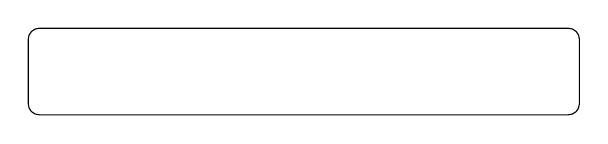
\begin{tikzpicture}
\draw[rounded corners] (0,0) rectangle (7,1.1);
\end{tikzpicture}}

\margin{e) Si $f\in\Gamma(U,\mathcal{E}_U)$, le morphisme
$g\mapsto G(f,g)$ de $\mathcal{E}_U$ dans $\underline{\omega}_U^{\otimes2}$ est
un épi.}

\textcircled{II} Si, au lieu de prendre $X$ fixe, on prend $X$ variable,
avec \unsure{morphismes|compatibilités} étales entre des $X$, on a
$=$ résultat, et l'indétermination sera
\[
G'=cG\qquad c\in\mathbb{C}^{*}\quad !
\]

\margin{Ici, au lieu des \unsure{la condition|conditions} d) e)
il suffit de supposer d)
\deleted{\unsure{de groupe} \unsure{additif|trivial}}.}
\figure{\begin{tikzpicture}
\draw[rounded corners] (0,0) rectangle (4.8,2.2);
\draw (0.2,2.15) .. controls (-0.3,2.6) and (-0.5,2.3) .. (-0.3,2.1);
\end{tikzpicture}}

\scanpage{73}
% archive foliation: 72
[Ici, on montre que \inserted{la condition a) implique que}
pour $\forall X$ fixé, l'expression de a),
$G(f,g)=R(f,f',\ldots,f^{(n)};g,g',\ldots,g^{(n)})$ doit avoir
des coefficients $\in\mathbb{C}$, \unsure{indépendante|indépendants} de $X$, donc
\[
R\in\mathbb{C}(F_0,F_1,\ldots,F_n;G_0,\ldots,G_n)
\]
et en fait,
\[
R(\quad)=
\underbrace{P(F_0,\ldots;G_0,\ldots)}_{\in\mathbb{C}[F_0,\ldots,G_n]}
/F_1^pG_1^q
\]
]

On peut prendre
\[
G(f,g)=\bigl(
\left[-2\frac{g'''}{g'}+3\left(\frac{g''}{g'}\right)^2\right]
-\left[-2\frac{f'''}{f'}+3\left(\frac{f''}{f'}\right)^2\right]
dt^2
\]

De plus, on trouve un torseur canonique $\mathcal{T}_X$ \unsure{sous}
$\underline{\omega}_{X/\mathbb{C}}^{\otimes2}$,
dépend \unsure{fonctiellement|fonctoriellement} de $X$ (pour morphismes
étales), et
\[
\deleted{\unsure{\varphi}}\ c^X:\mathcal{P}_X\longrightarrow\mathcal{T}_X
\]
tel que
\[
\left\{\begin{array}{l}
G(f,g)=c^X(g)-c^X(f)\\
c^X\text{ se factorise en }H\backslash\mathcal{P}_X\longrightarrow\mathcal{T}_X\\
\text{ce dernier morphisme est un iso}
\end{array}\right.
\]

III) On prend maintenant $X$ \inserted{schémas} variable lisse
(\unsure{en} \unsure{gardant|grandes} diff. \unsure{lim.} à l'ordre $2$)
sur des schémas variables, et on cherche pour tt tel $X$
\diagram{\begin{tikzcd}
\mathcal{E}_X\times\mathcal{E}_X \arrow[r,"G"] & \omega_{X/S}^{2}
\end{tikzcd}}
de façon compatible aux chgt de base $S'\longrightarrow S$,
aux morphismes étales
\diagram{\begin{tikzcd}
X' \arrow[r] \arrow[dr,no head] & X \arrow[d,no head]\\
& S
\end{tikzcd}}
et satisfaisant aux conditions qui correspondent à a), b), c),
(\uline{plus} la condition d) \deleted{\unsure{e)}}
\inserted{si \deleted{\unsure{on}} $S$ corps de car. $0$, et e) dans}
\deleted{``\unsure{formulation possible} analytique complexe''}.

\margin{la \unsure{forme suivante}:
$G(f,g)$ \unsure{non identiquement|non ident.}
nul en \unsure{car.} $\unsure{p>0}$.}
\figure{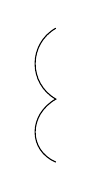
\begin{tikzpicture}
\draw (0,1.7) .. controls (-0.35,1.5) and (-0.35,1.0) .. (0,0.8)
.. controls (-0.35,0.6) and (-0.35,0.15) .. (0,0);
\end{tikzpicture}}

Mais quand on parle ``d'op. différentiel'', il faut maintenant remplacer
un polynôme $R$ en $f,f',f'',\ldots,g,g',g'',g'''$ par un
polynôme en
$f,f'=D_t^{(1)}f,D_t^{(2)}(f)\ldots D_t^{(n)}f,
g,g'=D_t^{(1)}g,D_t^{(2)}g,\ldots D_t^{(n)}g$.
\unsure{On voit clairement} à priori, les coeff.
sont dans $\Gamma(U,\underline{\mathcal{O}}_U)$
(où $t$, l'uniformisant, est défini sur $U$)
mais si on \deleted{\unsure{f}} en fait varier $X$, on
voit que les coefficients doivent être dans \uline{$\mathbb{Z}$}
(ou dans $\Gamma(S_0,\mathcal{O}_{S_0})$ si on a fixé un schéma de base
commun $S_0$ pour les $S,X\ldots$).
On trouve encore l'existence d'un tel, et l'unicité
à un facteur $\varepsilon\in\mathbb{Z}^{*}$ près, i.e. $\varepsilon=\pm1$:
\uline{unicité au signe près}! Ici on ne peut
prendre l'expression $G(f,g)$ précédente, car elle est
identiquement nulle en car. $2$ et $3$! Il faut
prendre $\frac1{12}G(f,g)$, savoir
\[
G_0(f,g)=\left[
\left(-\frac{D_t^{(3)}g}{D_t^{(1)}g}
+\left(\frac{D_t^{(2)}g}{D_t^{(1)}g}\right)^2\right)
-\left(-\frac{D_t^{(3)}f}{D_t^{(1)}f}
+\left(\frac{D_t^{(2)}f}{D_t^{(1)}f}\right)^2\right)
\right]dt^2
\]

Pour \unsure{caractériser} ce choix (parmi les deux
possibles au signe près) \unsure{on se cale} p.ex.
\[
G_0(t,t^2)=\deleted{\unsure{\frac1{2t}dt^2|\frac1{(2t)^2}dt^2}}
\frac1{2t}dt^2\qquad
(\text{au lieu de }-\frac1{2t}dt^2)
\]
[Il ne faut pas s'effrayer des dénominateurs, parce que
\unsure{là où} $2$ n'est pas inv. sur $X$: alors $t^2$ n'est jamais
un uniformisant!] ou si on veut quelque chose
qui ait un sens aussi en car. $2$
\[
G_0(t,t^3)=
\underbrace{\left(-\frac1{3t^2}+\left(\frac{3t}{3t^2}\right)^2\right)}_
{\frac1{t^2}(-\frac13+1)}dt^2
=\deleted{\unsure{\frac1{3t^2}}}+\frac23\frac1{t^2}dt^2
\]
[mais c'est inutile, car en car. $2$ les \deleted{\unsure{différents}}
\inserted{deux choix} possibles sur $\mathbb{Z}$ coïncident!].

\uline{\unsure{Remq.|Rem.}} 1) On peut se demander quel est le rôle joué dans
cet énoncé par les \unsure{biformes}, et s'il n'y aurait pas
moyen d'éliminer ce rôle. On est alors conduit,
dans I), à se donner un faisceau analytique
coh. $\mathcal{F}$ sur $X$, et à supposer
$G'\deleted{\unsure{(f,g)}}:\mathcal{E}_X\times\mathcal{E}_X\longrightarrow\mathcal{F}$.
On trouve alors qu'un tel $G'$ s'écrit de façon unique
(si $G$ est comme dans l'énoncé habituel, p.ex. celui de
II)) comme $G'=uG$, où $u:\underline{\omega}_X^{\otimes2}\longrightarrow\mathcal{F}$,
\unsure{et $u$ est} même un \uline{iso}!
Donc $\underline{\omega}_X^{\otimes2}$ joue ici un rôle \uline{universel}.
Dans II) on pourrait se donner un $\mathcal{F}_X$ \unsure{dépen-}

\scanpage{74}
% archive foliation: 73
\unsure{fonctorielle|fonctoriellement} de $X$, mais on trouverait encore
un iso fonctoriel en $X$, $\mathcal{F}_X\simeq\underline{\omega}_{X/\mathbb{C}}^{\otimes2}$.
De $=$ dans (III). Ainsi les $2$-formes sont essentielles.

2) \deleted{\unsure{G}} Le torseur $\mathcal{T}$ dont il est question dans
II (et \unsure{encore|a fortiori} dans I) dépend du choix de
$G$ (et de $\mathcal{F}$, si on veut --- c'est alors un
torseur sous $\mathcal{F}$) mais les \inserted{torseurs associés aux} différents choix
sont can. (semi)-isomorphes, de façon précise
\diagram{\begin{tikzcd}
\mathcal{T}^{G} \arrow[r,"\sim"] & \mathcal{T}^{\varphi G}\\
\underline{\omega}_X^{\otimes2} \arrow[r,"\varphi.\mathrm{id}"] &
\underline{\omega}_X^{\otimes2}
\end{tikzcd}}
\unsure{resp. aux}
i.e. $\mathcal{T}^{\varphi G}$ est ``multiple'' de $\mathcal{T}^{G}$ par $\varphi$.
Ainsi, le choix ``le plus fin'' de $\mathcal{T}$ est $\mathcal{T}^{G_0}$
(où $G_0$ est défini en (III)), alors le $\mathcal{T}^{G}$
correspondant au \inserted{$G$} \unsure{choisi|choix} de (II) est un
multiple $12$ième de $\mathcal{T}^{G_0}$.

3) On peut se \deleted{demander}\inserted{poser} la question
de caractériser $G_0(f,g)$ \uline{en une caractéristique donnée} $p>0$.
On peut prendre les conditions
a) b) c), \inserted{\unsure{vues} comme plus haut}, plus d') que $G_0(f,g)$ n'est pas id. nul
--- \uline{cela caractérise} $G_0(f,g)$ à multiplication près
par une constante $c\in\mathbb{F}_p^{*}$.
$\bar{M}$ \unsure{précisé|précisément} si
on a fixé un schéma de base absolu
\uline{intègre} $S_0$ (pour les $S$ et les $X$), l'indétermination
est dans $\Gamma(S,\mathcal{O}_S^{\unsure{\times|*}})$.
Si $S$ n'est pas intègre, il faut supposer que, sur chaque
$\unsure{k(s)|\kappa(s)}$, l'op. induit (pour des $X$ lisses
\deleted{\unsure{sur le}}\inserted{de dim. rel. $1$} sur $k(s)$)
\inserted{n'est pas identiquement nul.}

\margin{\uline{faux?} \unsure{pour un|vrai si}
\unsure{op.|W'} \unsure{diff.} d'ordre $\leq3$)}
\figure{\begin{tikzpicture}
\draw (0,0) -- (0,3.1);
\draw (0,1.1) -- (-0.6,1.1);
\draw (-0.6,1.1) circle (0.06);
\draw (0.2,0) .. controls (0.7,-0.4) and (0.8,-0.7) .. (0.2,-0.9);
\end{tikzpicture}}

\scanpage{75}
% archive foliation: 74
Les développements précédents étaient centrés
sur le groupe $H=GP(1,\mathbb{C})$ agissant sur $\mathbb{P}^{1}(\mathbb{C})$
(ou $GP(1)_{\mathbb{Z}}$ sur $\mathbb{P}^{1}_{\mathbb{Z}}\ldots$), et les invariants
différentiels, sous l'action de ce groupe, des
fonctions analytiques complexes (\uline{NB} \unsure{tout cela}
vaut aussi dans l'analytique réel, ou le
$C^{\infty}$, ou $C^3$).
On va passer rapidement en revue les développements
analogues pour d'autres groupes

a) \uline{Groupe des translations} $G_a$ \uline{agissant sur $\unsure{\underline{E}^{1}|\underline{A}^{1}}$}

On a l'opération (dans l'analytique complexe
p.ex.)
\[
d:\underline{\mathcal{O}}_X\longrightarrow\underline{\Omega}^{1}_{X/\mathbb{C}}
=\underline{\omega}_X
\]
qui \inserted{épi ($X$ lisse dim $1$) et}
s'annule exactement sur les fonctions
loc. constantes, donc vient
\[
A(f,g)=dg-df,\qquad
A:\underline{\mathcal{O}}_X\times\underline{\mathcal{O}}_X
\longrightarrow\underline{\omega}_X
\]
\margin{Ici $\underline{\mathcal{O}}_X$ \unsure{mauvais};
\unsure{prendre} $\mathcal{E}_X$ plutôt!}

on trouve l'analogue de a) b) dessus,
plus
\[
A(f,g+c)=A(f,g)\qquad c\in\mathbb{C}
\]
plus
\[
A(f,g)=A(f,h),\quad g(x)=h(x)\quad\Longrightarrow\quad
\underset{\text{au vois. de }x}{g=h}
\]
et
\[
g\longmapsto A(f,g)\qquad
\mathcal{E}_X\longrightarrow\underline{\omega}_X\quad\text{épi}
\]
(Cas $X$ lisse de dim $1$ \unsure{p. sûr|p. ass.}) ---

Ici pas la peine d'introduire de torseur,
\inserted{(sinon, il est trivial)}
\unsure{$\omega$|un} $=$ $A(f,g)$, \unsure{car} l'expression
des \unsure{lettres} \unsure{telles} qui en \unsure{occurrent|sortent}

\scanpage{76}
% archive foliation: 75
Si on s'intéresse à $\mathcal E_X$ au lieu de $\underline{\mathcal O}_X$,
il faut remplacer $\underline\omega_X$ par $\underline\omega_X^*$
(\unsure{donc} faisceau des bases de $\underline\omega_X$, i.e. des
\unsure{sects|sections} sans zéros), qui est un torseur
\uline{sous $\underline{\mathcal O}_X^*$}, et $dg-df$ par
\deleted{$\unsure{dg}$} :
\[
A'(f,g)=\frac{dg}{df}\in\Gamma(X,\underline{\mathcal O}_X^*)
\]

b) $G_m$ \uline{agissant sur $\underline E^1$, ou
$\underline E^{1*}\simeq G_m$} par \deleted{translations}
\inserted{homothéties}. Plus \unsure{généralement|général.}, considérons
son opération sur un faisceau inversible $L$, soit $L^*$ le sous faisceau
des bases \inserted{(torseur sous $\underline{\mathcal O}_X^*$)},
on s'intéresse à $L^*/\mathbb C^*$. Or à tt section de $L^*$ est associée
une connexion sur $L$ : on trouve ainsi un hom
\[
L^*\deleted{\unsure{f}}\xrightarrow{D}
\underline{\operatorname{Conn}}_{X/\mathbb C}(L^*)
\qquad(f\longmapsto D_f)
\]
où le dernier est un torseur sous
$\unsure{\underline\Omega^1_{X/\mathbb C}|\underline\omega_{X/\mathbb C}}$,
et ceci induit un \deleted{biject} iso
\[
L^*/\mathbb C^*\simeq\underline{\operatorname{Conn}}_{X/\mathbb C}(L).
\]

Si on ignorait la notion de connexion, on introduirait directement
$B(f,g)$ $(f,g\in\Gamma L^*)$, qui se \unsure{conf.|confond} $D_g-D_f$, par
\[
B(f,g)=\frac{d\,g/f}{g/f}\in\Gamma\underline\omega_{X/\mathbb C}
\]
avec des propriétés du type a) b) c) d) e). Dans le cas
$L=\underline{\mathcal O}_X$,
$\underline{\operatorname{Conn}}(L)\simeq\underline\omega_{X/\mathbb C}$
can., et il suffit de considérer
\[
g\longmapsto\frac{dg}{g}\qquad
\mathcal O_X^*\longrightarrow\underline\omega_{X/\mathbb C}
\]
qui induit
\[
\frac{\underline{\mathcal O}_X^{\unsure{\prime|*}}}{\mathbb C^*}
\simeq\underline\omega_{X/\mathbb C}.
\]
\figure{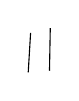
\begin{tikzpicture}[x=1cm,y=1cm]
\draw (0,0)--(0.03,0.50);
\draw (0.27,0.02)--(0.28,0.56);
\end{tikzpicture}}

\scanpage{77}
% archive foliation: 76
On a aussi : $B'(f,g)=\dfrac{dg}{g}-\dfrac{df}{f}$, \unsure{\ldots}

Si on veut par contre un invariant sur $\mathcal E_X^{\deleted{*}}$, on prendra
\[
g\longrightarrow\frac{g}{dg}\qquad
\mathcal E_X\longrightarrow\underline\omega_{X/\mathbb C}^{\otimes(-1)}
\]
on \deleted{trouve} \unsure{définit}
\[
\unsure{C|B}^{\unsure{!|\prime}}(f,g)=
\deleted{\frac{dg}{g}-\frac{df}{f}}
g(dg)^{-1}-f(df)^{-1}
\]
satisfaisant à a) b) c)
$[C^{\unsure{?|\prime}}(f,g)=C^{\unsure{?|\prime}}(f,ag)$
si $a\in\mathbb C^*)$
d) $(C^{\unsure{?|\prime}}(f,g)=C^{\unsure{?|\prime}}(f,h)$ et
$g(x)=h(x)$ en \uline{un pt qui n'est pas un zéro} de $g$ ou $h$
$\Longrightarrow g=h]$ et e) \deleted{$g\longmapsto C(f,g)$}
\unsure{pas tenu|pas très} : \unsure{faux e|fait e}, car
\deleted{$g(dg)^{-1}-f(df)^{-1}$}
p.ex. $g(dg)^{-1}$ ne peut être id. nul si $g\in\Gamma \mathcal E_X$ !
Donc il faut se borner à
$\mathcal E_X^*\inserted{=\widetilde{\operatorname{Et}}_{\mathbb C.\mathrm{an}}
(X,\mathbb C^*)}$, auquel cas on l'envoie dans
$\underline\omega_{X/\mathbb C}^{\otimes(-1)*}$ par $g(dg)^{-1}$,
ou aussi dans $\underline\omega_{X/\mathbb C}^*$ par $dg/g$,
et il y a lieu de considérer $\omega_{X/\mathbb C}^*$ comme un torseur
sous $\underline{\mathcal O}_X^*$.

Donc ici on prendra
\[
C^{\unsure{?|\prime}}(f,g)=\frac{dg}{g}:\frac{df}{f}
=\frac{dg}{df}\frac{g}{f}\in\Gamma(X,\underline{\mathcal O}_X^*)
\]

Dans tous ces cas, l'espace des valeurs \unsure{par|prises par} les $f,g$
\inserted{$(\mathbb P^1(\mathbb C),\underline E^1(\mathbb C),G_m(\mathbb C))$}
\unsure{étant} un \uline{espace homogène} sous le groupe d'op.
envisagé $(\unsure{GP(1)|Gb(1)},G_a,G_m)$ ce qui semble
\unsure{condition} de succès ($G_m$ opérant sur $\mathbb C$ : mauvais !)

c) Groupe $\operatorname{Aff}(1)$ \deleted{$\unsure{G}$}
$=G_m\mathbin{.}G_a$ opère sur $\underline E^1$.

On considère donc
\figure{\begin{tikzpicture}[x=1cm,y=1cm]
\draw (0,0)--(0,0.58);\draw (0.25,0.04)--(0.24,0.61);
\end{tikzpicture}}

\scanpage{78}
% archive foliation: 77
\diagram{\begin{tikzcd}[column sep=small,row sep=small]
\mathcal E_X\arrow[rr]\arrow[dr]&&\underline{\operatorname{Conn}}(\underline\omega_X)\\
&\underline\omega_{X/\mathbb C}^*\arrow[ur]&
\end{tikzcd}}
par $f\longrightarrow D_{df}$ ($=$ connexion de $\underline\omega_X$
pour laquelle \inserted{\unsure{aussi|ainsi}} $df$ est
\unsure{horizontale|horizontal})

on trouve
\[
\operatorname{Aff}(1,\mathbb C)\backslash \mathcal E_X
\simeq\underline{\operatorname{Conn}}(\omega_X)
\]
car successivement par a)
\[
G_a(\mathbb C)\backslash \mathcal E_X\overset{d}{\simeq}\underline\omega_X^*
\]
et par b)
\[
G_m(\mathbb C)\backslash\underline\omega_X^*
\overset{\sim}{\longrightarrow}\underline{\operatorname{Conn}}(\omega_X)
\]
On trouve donc
\[
D(f,g)=\frac{d\,\dfrac{dg}{df}}{\dfrac{dg}{df}}
\in\Gamma\underline\omega_X
\]
Si on a \unsure{unif\textsuperscript{te}|unif\textsuperscript{le}} $t$, cela fait
\[
D(f,g)=\frac{d\,\dfrac{g'}{f'}}{\dfrac{g'}{f'}}
=\frac{dg'}{g'}-\frac{df'}{f'}
=\left(\frac{g''}{g'}-\frac{f''}{f'}\right)dt
\]

\deleted{\unsure{cas spécial}}

d) \deleted{$\unsure{\mathcal E_X}$} \uline{Groupe} ``\uline{affine}'' \uline{de} $G_m$
\[
\underset{\substack{\Vert\\\mathbb Z/2\mathbb Z}}{\operatorname{Aut}(G_m)}
\mathbin{.}G_m
\]
\uline{opérant sur $G_m$.} ?
\[
f\longmapsto\frac1f\quad\text{et}\quad
f\unsure{\mathrel{\mid\!\!-\!\!-}|\longmapsto}cf
\quad(c\in\mathbb C^*)
\]
$f$ dans $\underline{\operatorname{Et}}(X,\mathbb C^*)
\unsure{\mathrel{=:}|=}\mathcal E_X^*$. On prend
\diagram{\begin{tikzcd}[column sep=small,row sep=small]
\mathcal E_X^*\arrow[rr]\arrow[dr,"{f\mapsto df/f}"']&&
(\underline\omega_X^{\otimes2})^*\\
&\underline\omega_X^*\arrow[ur,"{\omega\mapsto\omega^2}"']&
\end{tikzcd}}

\scanpage{80}
% archive foliation: 79
$\omega$ base de $\underline\omega^{\otimes n}$ $(n\in\mathbb Z,n\ne0)$

$\omega^{1/n}$ base de $\underline\omega$ définie loc. \unsure{mod} mult.
par $\varepsilon$, $\varepsilon^n=1$

$\int\omega^{1/n}$ bien défini mod transformations
$f\longmapsto\varepsilon f+b$ $(\unsure{\varepsilon\equiv1|\varepsilon^n=1})$
\inserted{donc $c_{\int\omega^{1/n}}$ bien défini}

Si $t$ uniformisante et $\omega=f(t)dt^n$, on aura
\[
\omega^{1/n}=f^{1/n}dt\quad\text{et}\quad
\deleted{\unsure{c_{\int\omega^{1/n}}}}
c_{\int\omega^{1/n}}=c_{\int f^{1/n}dt}\deleted{=c_t+}
\]
\[
c_n(\omega)=c_t+\left[-\frac2n\frac{f''}{f}
+\frac{2n+1}{n^2}\left(\frac{f'}f\right)^2\right]dt^2
\qquad\text{si }n\ne0
\]

\deleted{$\unsure{Gc_n(\omega)}$}
\[
\begin{aligned}
G_{m,n}\left(
\underset{\substack{\Vert\\f(dt)^m}}{\omega_m},
\underset{\substack{\Vert\\g(dt)^n}}{\unsure{\omega'_n|\omega_n}}\right)
&=c_n(\unsure{\omega'_n|\omega_n})-c_m(\omega_m)\\
&=\left[\left(-\frac2n\frac{g''}{g}
+\frac{2n+1}{n^2}\left(\frac{g'}g\right)^2\right)\right.\\
&\unsure{-}\qquad\left.-\left(-\frac2m\frac{f''}f
+\frac{2m+1}{m^2}\left(\frac{g'}g\right)^2\right)\right]dt^2
\end{aligned}
\]
\[
\left\{\begin{aligned}
G_{m,n}(\omega_m,\omega'_n)+G_{n,\unsure{r|p}}(\omega'_n,\omega''_p)
&=G_{m,p}(\omega_m,\omega''_p)\\
G_{m,n}(\omega_m,\omega_n)&=G_{m,nr}(\omega_m,\omega_n^r)
\quad\text{si }n\ne0,\ r\ne0\\
G_{m,n}(\omega_m,ds)&=G_{m,0}(\omega_m,s)\\
G_{0,0}(t,s)&=G(t,s)
\end{aligned}\right.
\]
\inserted{\[
G_{m,n}(\omega_m,(ds)^n)=G_{m,0}(\omega_m,s)
\]}
\figure{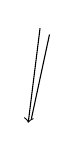
\begin{tikzpicture}[x=1cm,y=1cm]
\draw[->] (0.15,1.2)--(0,0);\draw (0.27,1.12)--(0.04,0.05);
\end{tikzpicture}}
\[
G_{m,n}((dt)^m,(ds)^n)=G_{0,0}(t,s)
\]
\margin{$c'_n(\omega)=n^2\dfrac{c_n(\omega)}{\deleted{\unsure{12}}}
\in\mathcal T_X^{\unsure{\otimes|*}n^2}$}

\deleted{$c'_n(\omega)$}\qquad $m,n\qquad
\delta=m\alpha=n\beta\qquad\delta^2=m^2\alpha^2=n^2\beta^2$
\[
\begin{aligned}
\omega_m\longmapsto{}&\alpha^2\deleted{\unsure{c}}c'_m(\omega_m)
=\alpha^2m^2\frac{c_m(\omega_m)}{12}
\deleted{\unsure{\in\Gamma\mathcal T_X^{\otimes\delta^2}}}\\
&=\frac{\delta^2c_m(\omega_m)}{12}
\in\Gamma\mathcal T_X^{\unsure{\otimes|*}\delta^2}
\end{aligned}
\]
\[
\omega'_n\unsure{\mathrel{\mid\!\!-\!\!-}|\longmapsto}
\beta^2c'_n(\omega'_n)
=\beta^2n^2\frac{c_n(\omega'_n)}{12}
=\delta^2\frac{c_n(\omega'_n)}{12}
\in\Gamma\mathcal T_X^{\unsure{\otimes|*}\delta^2}
\]
\[
G'_{m,n}(\omega_m,\omega'_n)=\alpha^2c'_m(\omega_m)-\beta^2c'_n(\omega'_n)
\in\Gamma\mathcal T_X^{\unsure{\otimes|*}\delta^2}
\]
\[
\left\{\begin{aligned}
\unsure{G_n|G}(t,as)&=G(t,s)&a&\in\Gamma(S,\mathcal O_S^*)\\
G(t,s+b)&=G(t,s)&b&\in\Gamma(S,\mathcal O_S)\\
G(t,1/s)&=G(t,s)&s&\in\operatorname{Et}_S(X,G_{m,S})
\end{aligned}\right.
\]

% The following calculations are written upside down at the foot and lower right.
\margin{\[
\begin{gathered}
f\longmapsto af+b\qquad df=dg\Longrightarrow G(f,g)=0\\
f\longmapsto af\qquad
\left(\frac{df}{f}\right)^2=\left(\frac{dg}{g}\right)^2
\Longrightarrow G(f,g)=0\\
df\qquad\left(\frac{df}{f}\right)^2\qquad
(df-dg)\left(\left(\frac{df}{f}\right)^2-
\left(\frac{dg}{g}\right)^2\right)\\
\frac{df}{f}=c\frac{dg}{g}\qquad ?\\
\log f=c\log g\\
f=g^c
\end{gathered}
\]}
\figure{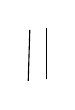
\begin{tikzpicture}[x=1cm,y=1cm]
\draw (0,0)--(0.02,0.65);\draw (0.23,0.02)--(0.23,0.67);
\end{tikzpicture}}

\scanpage{81}
% archive foliation: 80
\diagram{\begin{tikzcd}[column sep=small,row sep=small]
D_X\arrow[r,leftrightarrow,"{\mathbb R\text{-an}}"]&
U(x)\arrow[r,phantom,"{\overset{\mathrm{Can}}{\unsure{\hookrightarrow|\leftrightarrow}}}"]\arrow[d]&
B(x)\arrow[r,phantom,"{\overset{\mathrm{Can}}{\unsure{\hookleftarrow|\leftrightarrow}}}"]
\arrow[d,phantom,"{\unsure{\mathbb R\text{-an}}}"]&
V(x)\arrow[r,Rightarrow,"{\mathbb R\text{-anal.}}"]&
\deleted{\unsure{E}}\unsure{D'_X|D_X}\arrow[d]\\
&X_X&\Sigma(x)\arrow[d,bend left=18,no head]&&\bar X_X\\
&&\widehat T_X\arrow[u,bend right=8,no head,"{\mathbb R\text{-an}}"',"{?}"]&&
\end{tikzcd}}
\margin{$D_{\unsure{x|n}}\subset T_{X,x}
\deleted{\unsure{\longleftrightarrow}}\supset
\underset{\substack{\unsure{\Vert|21}\\\bar D_x}}{D'_a}$}

\[
\widetilde X_{(x)}\mathbin{\times}_{(X;\unsure{\Pi(x)|\Pi_1(x)})}
\widetilde{\bar X}_{(x)}=
\qquad\deleted{\unsure{R}}
\]
\[
X(x)\qquad\Pi_1(X,x)
\]
\unsure{rev\textsuperscript{ts} droits}
\[
\widetilde X\qquad\Pi_x\times\Pi_{\unsure{x|n}}
\]

\diagram{\begin{tikzcd}[column sep=large,row sep=small]
\bar X_X&\Sigma(x)&\bar X_X\\
U(x)\arrow[u,"{\mathbb C\text{-an}}"]
\arrow[d,"{\mathbb R\text{-anal.}\;?}"']&
B(x)\arrow[l]\arrow[r]\arrow[u]
\arrow[d,"{?\;\mathbb R\text{-anal.}}"]&
V(x)\arrow[u]\arrow[d,"{?\;\mathbb R\text{-anal.}}"]\\
D_X\arrow[d,"{\deleted{\unsure{\xi}}}"]&
\widehat T_X\arrow[l]\arrow[r]\arrow[d]&D'_X\\
{}&\substack{\Sigma_X\\=}&
\end{tikzcd}}

\[
\unsure{\widehat T_X^*|\widehat{\mathcal T}_X^*}+\mathcal O_X
\]
\[
\unsure{\mathfrak g_X|\mathcal T_X}+\underline{\mathcal O}_X
=\Omega^{-1}\oplus\Omega^0
\]
$GP(1,\mathbb C)$

$B(x)_y=$ \unsure{cl.m d'équivo.|cl. d'équiv.} de couples $(c,\xi)$
\[
\xi\in\widehat T_{X,a}\qquad c\in\Pi(a,y)
\]
\[
(c\lambda,\xi)\simeq(c,\lambda\xi)
\qquad(\lambda\in\Pi(a))
\]

\[
\check E\otimes E=(\Omega^1+\Omega^0)\otimes(\Omega^{-1}\oplus\Omega^0)
\qquad\deleted{(\unsure{h},\xi}
\]
\diagram{\[
=\begin{pmatrix}\Omega^0&\Omega^{-1}\\\Omega^1&\Omega^0\end{pmatrix}
\]}
\diagram{\[
\underline{\check E\otimes E}\otimes\Omega^1\simeq
\begin{pmatrix}\Omega^1&\Omega^0\\\Omega^2&\Omega^1\end{pmatrix}
\]}
\diagram{\[
\deleted{\begin{pmatrix}\unsure{1|a}&0\\\unsure{2g+2|2g-2}&\unsure{1|a}\end{pmatrix}}
\qquad\deleted{2g}\qquad
\unsure{\mathfrak g|\mathcal G}\otimes\Omega^1\subset
\begin{pmatrix}\Omega^1&\Omega^0\\\Omega^2&-\Omega^1\end{pmatrix}
\]}

\[
f,g\qquad a^2=1\qquad a=\pm1\qquad g+1
\]
\diagram{\[
\begin{array}{cc|c}
3g-3&1&4g-2\\
\deleted{\unsure{2}}\unsure{+|:}g&&
\end{array}
\]}
\[
f+\frac1f=\qquad\Omega^1=\omega^{\otimes2}
\qquad\unsure{g=-f\,df|g=-\int df}
\]
\[
\frac{f^2+1}{f}
\]
$\unsure{\varphi|f}$ \uline{sans zéro}
\[
\deleted{\unsure{a}}\qquad\frac g{g'}=\varphi
\qquad\frac{g'}g=\frac1\varphi
\]
\[
f\longmapsto\frac1f\quad/\quad
f+\frac1f=\frac{f^2+1}{f}=h\qquad h\ \text{sans zéro.}
\]
\[
f^2-fh+1=
\]
\[
\log g=\int\frac1\varphi+\qquad
g=c\exp\int\frac1\varphi
\]
\figure{\begin{tikzpicture}[x=1cm,y=1cm]
\draw (0,0.2)--(5.2,5.7);
\draw (1.4,-2.9)--(6.4,1.6);
\draw (2.9,0.4)--(4.1,1.55);
\draw (2.55,-2.15) .. controls (2.0,-1.95) and (2.1,-1.6) .. (1.9,-1.5);
\end{tikzpicture}}

\scanpage{82}
% archive foliation: 81
\uline{écart additif}
\[
A_1(f,g)=dg/df=\frac{g'}{f'}
\qquad A_n(f,g)=\left(\frac{dg}{df}\right)^n
=\left(\frac{g'}{f'}\right)^n
\]
\deleted{\unsure{écart}}

\uline{écart affine}
\[
\operatorname{Aff}(f,g)=D_{dg}-D_{df}
=\frac{d\,\dfrac{dg}{df}}{dg/df}
=\frac{d\,\dfrac{g'}{f'}}{g'/f'}
=\frac{dg'}{g'}-\frac{df'}{f'}
=\left(\frac{g''}{g'}-\frac{f''}{f'}\right)dt
\]
\diagram{\begin{tikzcd}[column sep=small,row sep=large]
& &\substack{\mathcal E_X/(\mu_n.G_a)(\mathbb C)
\overset{\sim}{\longrightarrow}\underline\omega_X^n\\
c_{a,n}(f)=(df)^n\\\text{torseur sous }\underline O_X^*}
\arrow[r,"{(n=0)}"]
&\substack{\mathcal E_X/(G_m.G_a)(\mathbb C)
\overset{\sim}{\longrightarrow}\operatorname{Conn}(\underline\omega_X^1)\\
c_{af}(f)=D_{df}\\\text{torseur sous }\underline\omega_X^1}
\arrow[d,"{D\mapsto c_D}"]\\
\mathcal E_X\arrow[r]\arrow[dd,dashed,"\exp"']
&\substack{\mathcal E_X/G_a(\mathbb C)\overset{\sim}{\longrightarrow}
\underline\omega_X^{1*}\\c_a(\deleted{\unsure{f}}f)=df\\
\text{torseur sous }\underline O_X^*}
\arrow[ur]\arrow[dd,bend right=14,"?"']\arrow[dd,bend left=14,"\mathrm{id}"]
&&\substack{\mathcal P_X/GP(1,\mathbb C)\overset{\sim}{\longrightarrow}
\operatorname{Conn\,proj}(X)\\c_{pr}(f)=c_{D_{df}}\\
\underline\omega_X^2\quad(\text{torseur sous})}\\
&&\substack{\mathcal E_X^*/(\mathbb Z/2\mathbb Z.G_m)(\mathbb C)
\simeq\underline\omega_X^{2*}\\\text{torseur sous }\underline O_X^*}&\\
\mathcal E_X^*\arrow[r]
&\substack{\mathcal E_X^*/G_m(\mathbb C)\overset{\sim}{\longrightarrow}
\underline\omega_X^{1*}\\c_m(f)=df/f\\
\text{torseur sous }\underline O_X^*}\arrow[ur]&&
\end{tikzcd}}
\margin{$\unsure{r|f}$;\quad\deleted{$\unsure{\mathcal E_X^*}$};\quad
\deleted{$\mathcal E_X\unsure{?}$};\quad $\mathcal E_X$}
\[
\underline O_X^*\xrightarrow{\varphi\mapsto\varphi^n}\underline O_X^*
\xrightarrow{\varphi\mapsto-\frac1n\frac{d\varphi}{\varphi}}
\underline\omega_X^1
\qquad
\underline O_X^*\xrightarrow{\varphi\mapsto\varphi^2}\underline O_X^*
\]
\[
\boxed{c_{D+\omega_1}=c_D+2D\omega_1+\omega_1^2}
\]
\figure{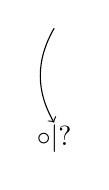
\begin{tikzpicture}[x=1cm,y=1cm]
\draw[->] (0,1.2) to[bend right=30] (0,0);
\node at (0,-.2) {$\unsure{\circ|?}$};
\end{tikzpicture}}
\[
\exp(\pm f+a)=\underline{\unsure{\exp a|e^a}}(\exp f)^{\pm1}
\]
\figure{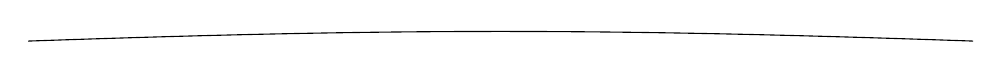
\begin{tikzpicture}\draw (0,0) to[bend left=2] (12,0);\end{tikzpicture}}

\[
\operatorname{Ecad}(f,g)=\frac{dg}{df}=\frac{g'}{f'}\in\Gamma\underline O_X^*
\]
\[
\unsure{\operatorname{Ecaf}_n|\operatorname{Ecad}_n}(f,g)
=\left(\frac{dg}{df}\right)^n=\left(\frac{g'}{f'}\right)^n
\in\Gamma(\underline O_X^*)
\]
\[
\operatorname{Ecaf}(f,g)=\frac{d(dg/df)}{dg/df}
=\frac{d(g'/f')}{g'/f'}=\frac{dg'}{g'}-\frac{df'}{f'}
=\left(\frac{g''}{g'}-\frac{f''}{f'}\right)dt
\in\Gamma(\underline\omega_X^1)
\]
\[
\operatorname{Ecmu}_1(f,g)=\frac{dg/g}{df/f}
=\frac{g'/g}{f'/f}\in\Gamma(\underline O_X^*)
\]
\[
\operatorname{Ecmu}_2(f,g)=\left(\frac{dg/g}{df/f}\right)^2
=\left(\frac{g'/g}{f'/f}\right)^2\in\Gamma(\underline O_X^*)
\]
\[
\begin{aligned}
\operatorname{Ecpr}(f,g)
&=-2\frac{d^3g/df^3}{dg/df}+3\left(\frac{d^2g/df^2}{dg/df}\right)^2\\
&=\left[\left(-2\frac{g'''}{g'}+3\left(\frac{g''}{g'}\right)^2\right)
-\left(-2\frac{f'''}{f'}+3\left(\frac{f''}{f'}\right)^2\right)\right]dt^2
\in\Gamma(\underline\omega_X^{\unsure{1|2}})
\end{aligned}
\]

\diagram{\begin{tikzcd}[column sep=small,row sep=large]
\mathcal E_X\arrow[r,"d"]\arrow[ddd,"\exp"']
&\left[\substack{\mathcal E_X/G_a(\mathbb C)\overset{\sim}{\longrightarrow}
\underline\omega_X^{1*}\\c_a(f)=df}\right]
\arrow[r,"\alpha_n"]\arrow[ddd,bend right=12,"?"']
\arrow[ddd,bend left=12,"\mathrm{id}"]
&\left[\substack{\mathcal E_X/(\mu_n.G_a)(\mathbb C)
\overset{\sim}{\longrightarrow}\underline\omega_X^{n*}\\c_{a,n}(f)=(df)^n}\right]
\arrow[r,"\beta_n"]\arrow[ddd,"{\mathrm{id}\ (n=2)}"]
&\left[\substack{\mathcal E_X/(G_m.G_a)(\mathbb C)\simeq
\operatorname{Conn}(\underline\omega_X)\\c_{af}(f)=D_{df}}\right]
\arrow[dd,"\gamma"]\\
&\underline O_X^*\arrow[r,"{\varphi\mapsto\varphi^n}"]\arrow[d,"\mathrm{id}"']
&\underline O_X^*\deleted{\unsure{\underline O_X^*}}
\arrow[r,"{\varphi\mapsto-\frac1n\frac{d\varphi}{\varphi}}"]
\arrow[d,"\mathrm{id}"']&\underline\omega_X\\
&\underline O_X^*\arrow[r,"{\varphi\mapsto\varphi^2}"']
&\underline O_X^*\arrow[r,bend right=15]
&\substack{[\mathcal P_X/GP(1,\mathbb C)\simeq\operatorname{Conn}(X)]\\
\underline\omega_X^2}\\
\mathcal E_X^*\arrow[r]
&\left[\substack{\mathcal E_X^*/G_m(\mathbb C)\simeq\underline\omega_X^{1*}\\
c_m(f)=df/f}\right]\arrow[r,"{\alpha'_2}"]
&[\mathcal E_X^*/(\mathbb Z/2\mathbb Z.G_m)(\mathbb C)\simeq\underline\omega_X^{2*}]
\arrow[ur,bend right=15,"\delta"']&
\end{tikzcd}}

\[
\alpha_n(\omega_1)=\omega_1^n
\]
\[
\begin{aligned}
\beta_n(\omega_n)&=\beta_1(\omega_n^{1/n})
=\beta_1(f^{1/n}dt)\\
&=D_{dt}\deleted{\unsure{\omega_1}}
+\unsure{-\frac1n|\frac1n}\frac{df}{f}
=D_{dt}+\unsure{-\frac1n|\frac1n}\frac{f'}f\,dt
\end{aligned}
\]
\margin{$\unsure{\beta_1(fdt)}$}
\[
\begin{aligned}
\gamma(D_{dt}+\underset{\Vert\ fdt}{\omega_1})
&=\underset{\Vert\ c_{pr}(t)}{\gamma(D_{dt})}
+2D_{dt}\omega_1+\omega_1^2\\
&=c_{pr}(t)+2\frac{df}{\unsure{dt}}dt+f^2dt^2
=c_{pr}(t)+(2f'+f^2)dt^2
\end{aligned}
\]
\[
\begin{aligned}
\gamma\beta_n(\omega_n)
&=c_{pr}(t)+\left(2\left(-\frac1n\frac{f'}f\right)'
+\left(-\frac1n\frac{f'}f\right)^2\right)dt^2\\
&=c_{pr}(t)+\frac1{n^{\unsure{2}}}
\left(-2n\frac{f''}f+\inserted{\unsure{(2n+1)}}
\deleted{\unsure{1}}\left(\frac{f'}f\right)^2\right)dt^2\\
&=c_{pr}(t)+\left(-2\frac{f''}f+3\left(\frac{f'}f\right)^2\right)dt^2
\end{aligned}
\]
\margin{$\gamma\beta_1(\omega_1)$}
\[
\gamma\beta_1d(f)=c_{pr}(t)+\deleted{\unsure{\frac1{n^2}}}
\left(-2\frac{f'''}{f'}+3\left(\frac{f''}{f'}\right)^2\right)dt^2
\]
\margin{\[
\begin{aligned}
\delta(\omega_2)&=\gamma\beta_2(\omega_2)+\omega_2\\
&=c_{pr}(\unsure{\omega_1|t})+
\left[f-\unsure{\frac{f''}f|2\frac{f''}f}+\frac54\left(\frac{f'}f\right)^2\right]dt^2\\
\delta\alpha'_2(\omega_1)&=\gamma\beta_1(\omega_1)
\deleted{\unsure{^{2}}}+\omega_1^{\unsure{2|1}}\\
&=c_{pr}(t)+\left[f^2-2\frac{f''}f+3\left(\frac{f'}f\right)^2\right]dt^2
\end{aligned}
\]}
\figure{\begin{tikzpicture}[x=1cm,y=1cm]
\draw (0,2) to[bend left=3] (0,0) to[bend right=3] (3,0);
\draw (.1,2)--(.1,.3);
\end{tikzpicture}}

\scanpage{83}
% archive foliation: 82
\[
\unsure{X|Y}=\Omega Y
\]
\diagram{\begin{tikzcd}[column sep=small,row sep=large]
k_1\arrow[r,phantom,"\in"]&H^3(\pi_1(X),\pi_2(X))\overset{?}{=}0\\
\exists\ k'_1\arrow[u,dashed]\arrow[r,phantom,"\in"]
&H^4(K(\pi_1(X),2),\pi_2(X)\arrow[u]\\
k''_1&H^5(K(\pi_1(X),3),\pi_2(X))\arrow[u]\\
&\unsure{\text{si}|\text{etc.}}\\
&H^{5+\unsure{r|q}}(K(\pi_1(X),3+\unsure{r|q},\pi_2(X))
\end{tikzcd}}

\diagram{\begin{tikzcd}[column sep=large,row sep=small]
&Y'\arrow[d]&\\
&K(\pi_1(X),2)\arrow[r,"{k'_1}"]&K(\pi_2(X),4)\\
&\unsure{\wr|\xi}&\\
S^1\wedge K(\pi_1(X),1)\arrow[r]&K(\pi_1(X),2)&
\end{tikzcd}}
\diagram{\begin{tikzcd}[column sep=large,row sep=large]
X=\Omega Y\arrow[d]&\\
K(\pi_1(X),1)\arrow[r,"k_1"]&K(\pi_2(X),3
\end{tikzcd}}

\scanpage{84}
% archive foliation: 83
donc
\[
\left(\frac{df}{f}\right)^2=\frac{(df)^2}{f^2}
=\left(\frac{f'\deleted{^{2}}}{f\deleted{^{2}}}\right)^2dt^2
\]
On a\quad a) b) c) d) e) --- On prendra
\[
E(f,g)=\left(\frac{dg}{g}\right)^2:
\left(\frac{df}{f}\right)^2
=\frac{\left(\dfrac{dg}{df}\right)^2}{(g/f)^2}
\]

\deleted{$\mathcal E_X/G_a(\mathbb C)\unsure{\mathcal E|\simeq}$}

\scanpage{86}
% archive foliation: 85
$X$ schéma.

1.1. Données équivalentes

a) fibré en droites projectives \inserted{$P$} sur $X$
(fibré de Br. Sev. de rang 1)
\[
f:P\longrightarrow X
\]
b) ``\unsure{Module|fibré} loc. libre \inserted{rang 2, $E$}
mod \unsure{tensorisation|association} par
modules inversibles'' sur $X$

c) Algèbre d'Azumaya \inserted{$M$} de rang 4
\margin{si 2 inv. sur $X$}

\[
\left\{\begin{array}{ll}
\text{d)}&\text{Algèbre de Lie }\mathfrak g\quad
\text{forme }\inserted{\text{(type)}}\text{ de }\mathfrak{gp}(1)_X\\
\text{d')}&\rule{3cm}{.3pt}\ \mathfrak g'\ \rule{2cm}{.3pt}\quad
\deleted{\unsure{\mathfrak{gp}}}\mathfrak{sl}(\unsure{1|2})_X
\end{array}\right.
\]
e) forme $G$ de $\underline{GP}(1)_X$

\deleted{\unsure{e'}} \unsure{e')|e\textsuperscript{bis})}
\rule{1cm}{.3pt} $G'$ de $\underline{SL}(2)_X$

Si on a $P$, on en déduit
\[
E=f_*(L),\quad \underline L\text{ module inv. sur }P
\text{ de degré 1 sur \unsure{ch.que|ch. une} fibre}
\]
($\underline L$ défini loc. fppf \inserted{sur $X$} ou loc ét., mod
tensorisation par $f^*(\lambda)$, $\lambda$ inv. sur $X$)
\[
M=\check E\otimes E\simeq\underline{\operatorname{End}}(E)
\simeq E\otimes E\otimes(\Lambda^2E)^{-1}
\]
ext. de
\[
\underline O_X\ (\simeq\Lambda^2E\otimes(\Lambda^2E)^{-1})
\quad\text{par}\quad\Gamma^2E\otimes(\Lambda^2E)^{-1}
\]
ext. de
\[
\operatorname{Sym}^2(E)\otimes(\Lambda^2E)^{-1}
\quad\text{par}\quad\underline O_X\ (\simeq\Lambda^2E\otimes(\Lambda^2E)^{-1})
\]
\inserted{\[
f_*(L^{\otimes2})\otimes(\Lambda^2E)^{-1}
\simeq f_*(\underbrace{L^{\otimes2}\otimes\unsure{f^*\Lambda^2E|f^*(\Lambda^2E)^{-1}}}_{\underline t_{P/X}})
\]}

\margin{\unsure{expliciter|expliquer} !; ]
\diagram{\begin{tikzcd}[row sep=small]
\operatorname{Sym}^2E\otimes\operatorname{Sym}^2E\arrow[d]\\
\operatorname{Sym}^2E\otimes\Lambda^2E
\end{tikzcd}}
et
\diagram{\begin{tikzcd}[row sep=small]
\Gamma^2E\otimes\Gamma^2E\arrow[d]\\
\Gamma^2E\otimes\Lambda^2E
\end{tikzcd}}
\unsure{et accouplements|et couplages}
formes de Killing
\diagram{\begin{tikzcd}[column sep=small,row sep=small]
\operatorname{Sym}^2E\otimes\operatorname{Sym}^2E\arrow[r]
&(\Lambda^2E)^{\unsure{\otimes2}}\\
\Gamma^2E\otimes\Gamma^2E\arrow[ur]&
\end{tikzcd}}}
\figure{\begin{tikzpicture}[x=1cm,y=1cm]
\draw (0,4)--(1,4.1) to[bend left=30] (2,3.4)--(1.4,.5)--(0,0);
\end{tikzpicture}}

\[
M\overset{?}{\simeq}f_*\bigl(P^1_{P/X}(\underline t_{P/X})\bigr)
\quad\unsure{\text{additivement}|\text{ad libitum}}\ ?
\]
\[
\mathfrak g=M/\underline O_X
\]
avec crochet déduit du crochet \inserted{$(xy-yx)$}
de $M$ [\uline{NB} $\underline O_X$ en est le centre]
\[
\simeq f_*(\underline t_{P/X})
\]
[avec crochet provenant du crochet dans $\underline t_{P/X}$]

\[
\mathfrak g'\subset M^{\unsure{=\,\ell|\ell}}
\]
sous-algèbre des éléments de trace réduite nulle

($\mathfrak g'\longrightarrow\mathfrak g$ can, iso si 2 inv. sur $X$)
\[
\Vert\qquad\mathfrak g'\subset\check E\otimes E^{\unsure{\ell}}
\]
sous-algèbre des él. de trace nulle

\[
G=\operatorname{Aut}_X P,\qquad
G'=\widetilde G\quad\text{(rev. univ. de Chevalley)}
\]
\[
=\deleted{\operatorname{Aut}}\underline{SL}(E)
\]
\margin{\[
\begin{aligned}
G&\simeq\underline{\operatorname{Aut}}(E)/G_{mX}\\
&\simeq\underline{\operatorname{Aut}}(M)\\
&\simeq\underline{\operatorname{Aut}}(\mathfrak g)\\
&\simeq\underline{\operatorname{Aut}}(\mathfrak g')
\end{aligned}
\]
! attention à la Car. (notamment Car. 2!)}
\figure{\begin{tikzpicture}[x=1cm,y=1cm]
\draw (2,2)--(0,0)--(1.7,1.3);
\draw (2.5,2.7) to[bend right=20] (2.7,1.5)
to[bend left=40] (3,.9) to[bend left=40] (2.7,.5)
to[bend right=20] (2.5,-.5);
\end{tikzpicture}}

$P=\mathbb P(E)=$ schéma des Idéaux à gauche
qui sont ``spéciaux'' i.e. loc. fact. directs et
``non \uline{\unsure{triviaux en aucun point|triviaux}}''
\deleted{\unsure{sur $X$}}

$=$ schéma des sous-Alg. de Borel de $\mathfrak g$
\figure{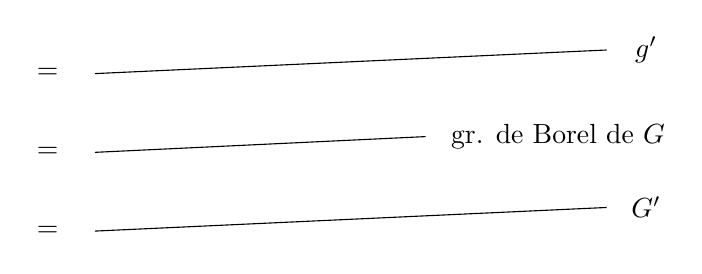
\begin{tikzpicture}[x=1cm,y=1cm]
\node at (0,2) {$=$};\draw (.6,2)--(7.1,2.3);\node at (7.6,2.3) {$\mathfrak g'$};
\node at (0,1) {$=$};\draw (.6,1)--(4.8,1.2);
\node[anchor=west] at (5,1.2) {gr. de Borel de $G$};
\node at (0,0) {$=$};\draw (.6,0)--(7.1,.3);\node at (7.6,.3) {$G'$};
\end{tikzpicture}}

\scanpage{87}
% archive foliation: 86; landscape manuscript on music paper
$E=$ module d'\unsure{une|un} ``rep. \unsure{vraie|naïve}''
\[
\begin{array}{ll}
\text{de}&\deleted{M}\ M\\
\text{de}&\mathfrak g\\
\text{de}&\mathfrak g'\\
\text{de}&G\\
\text{de}&G'
\end{array}
\qquad
\begin{array}{l}
\mathfrak g=\underline{\operatorname{Lie}}G\\
\mathfrak g'=\operatorname{Lie}G'
\end{array}
\]

1.2. Données équivalentes

a) fibré \deleted{\unsure{proj. $P$}} \inserted{en droites}
proj. $P$ sur $X$, avec section marquée $\sigma$

b) Structure d'extension
\[
0\longrightarrow\Omega\longrightarrow\mathcal L
\longrightarrow\underline O_X\longrightarrow0
\]
$\Omega$ inversible

c) Algèbre d'Azumaya de rg 4 $M$, avec idéal
\inserted{$\unsure{\mathfrak a}$} ``spécial''
$\unsure{\mathfrak a_\sigma|\mathfrak a}$

d) $\mathfrak g$ avec ss.-Alg. de Borel $\mathcal L$

\[
\begin{array}{llll}
\text{d')}&\mathfrak g'&\rule{4cm}{.3pt}&\mathcal L'\\
\text{e)}&G&\rule{1.8cm}{.3pt}\ \text{gr.}\ \rule{1.5cm}{.3pt}&B\\
\text{e')}&G'&\rule{1.8cm}{.3pt}\ \text{gr.}\ \rule{1.5cm}{.3pt}&B'
\end{array}
\]
\deleted{f) Une \unsure{$O_X$ Algèbre|Ext($O_X$)} avec une
\unsure{$P_2$|$\Omega_2$} \unsure{marquée}
\unsure{rigidité|rigidifiée} \unsure{d'extension 2|d'ordre 2},
de ``rang'' 1}
\inserted{\unsure{trivialisée|tr. qui est $e'$}}

\inserted{à a)} est associé $\unsure{L:=\underline L|\underline L}$
faisc. inv. de degré rel. $(1)$,
\uline{rigidifié} par $\sigma^*(L)\simeq\underline O_X$. Alors
\[
\begin{aligned}
+\quad\mathcal L&=f_*(L),\quad\text{avec structure d'ext. évidente}\\
&\simeq f_*\bigl(L/\unsure{\mathcal I^2L|\mathcal IL}\bigr)\\
&\simeq\sigma^*(P^1(L))
\end{aligned}
\]
($\mathcal I=$ Idéal de $\sigma(X)$ dans $P$)

$P=\mathbb P(\mathcal L)$ avec section corresp. au quotient
$\underline O_X$ de $\mathcal L$

$=$ clôture projective du torseur sous $W(\Omega)$ défini par l'extension.

et $M=\operatorname{End}\mathcal L$, avec idéal annulateur de $\Omega$
\margin{\deleted{(\unsure{formes splittées|formes déployées})}}
\[
\mathfrak g=M/\underline O_X\simeq\operatorname{Sym}^2(\mathcal L)
\otimes\Omega^{-1}\qquad(\mathrm{NB}\ \det\mathcal L\simeq\Omega)
\]
Or $\operatorname{Sym}^2\mathcal L$ est filtré par
\inserted{(décro)} $\underline O_X,\Omega,\Omega^2$,
donc $\operatorname{Sym}^2\mathcal L\otimes\Omega^{-1}$ filtré par (croiss)
\[
\begin{array}{ccc}
\Omega&\underline O_X&\Omega^{-1}\\
\Vert&\Vert&\Vert\\
\operatorname{Fil}_1&\operatorname{Fil}_2/\operatorname{Fil}_1
&\operatorname{Fil}_3/\operatorname{Fil}_2=\\
\Vert&\Vert&\Vert\\
\operatorname{gr}_1&\operatorname{gr}_2&\operatorname{gr}_3
\end{array}
\]
\figure{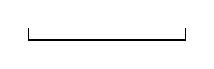
\begin{tikzpicture}\draw (0,.15)--(0,0)--(2,0)--(2,.15);\end{tikzpicture}}
\margin{\unsure{exprimer|expliquer} aussi \unsure{ce|de}
$(\mathfrak g,\mathcal L)$ \unsure{à partir|par}
\[
0\longrightarrow\Omega\longrightarrow\mathcal L
\longrightarrow\underline O_X\longrightarrow0
\]
$(\Omega=\mathcal L_{\unsure{\mathrm{un}}},\ldots)$}

% right-hand column, continuing the filtration computation
où
\[
\begin{aligned}
\operatorname{Fil}_2
&=\Omega^{-1}\otimes
\underbrace{(\operatorname{Ker}\operatorname{Sym}^2\mathcal L
\longrightarrow\operatorname{Sym}^2 O)}_{\simeq\Omega\otimes\mathcal L}\\
&\simeq\mathcal L
\end{aligned}
\]
donc on a
\[
\underset{\Omega}{\underbrace{\Omega}}\subset
\underset{\underline O_X}{\underbrace{\mathcal L}}\subset
\underset{\Omega^{-1}}{\underbrace{\mathfrak g}}
\]
et $\mathcal L$ est une ss.-Alg. de Borel
($\Omega$ \unsure{sa part.|rad.} unipotente)

\margin{\uline{NB} Pour forme de Killing,
$\Omega$ et $\mathcal L$ orth. l'un à l'autre, \inserted{2 inv.!}}

On n'explicite pas $(\mathfrak g',\mathcal L')$
($\simeq(\mathfrak g,\mathcal L)$ si 2 inv.), pour $(G,B)/(G',B')$ on a
\[
G'=\underline{SL}_{\Omega}\mathcal L,\qquad
B'\inserted{\subset G'}=\text{Stabilisateur de }\Omega
\]
$G,B$ déduits par passage au quot. par Centre $\mu_2$

\margin{\uline{NB}
\[
\mathfrak g/\Omega\simeq\unsure{\mathcal L^\vee|\mathcal L}
\]
\[
\mathcal L^\vee\simeq\mathcal L\otimes\det\mathcal L^{-1}
\simeq\mathcal L\otimes\Omega^{-1}
\]
avec filtration opposée

vérifier!}
\figure{\begin{tikzpicture}[x=1cm,y=1cm]
\draw (0,0) to[bend right=40] (-.5,2)
to[bend right=40] (2.3,2.6) to[bend right=40] (2.6,.5)
to[bend right=20] (0,0);
\draw[->] (2,3) to[bend left=25] (2.5,2);
\draw (2.3,2.6)--(4,2.6);
\end{tikzpicture}}

[\uline{1.\deleted{3}\inserted{4}.} Supposons $X/S$, et considérons des
\uline{connexions} \inserted{rel. $S$} sur les objets du type envisagé
dans 1.1, \unsure{mais augmentés|munis également}
\unsure{par} \inserted{la donnée d'}une structure 1.2.
Ainsi, on \unsure{consid.|considère} des couples
\[
(P,\sigma,C)
\]
\[
\left\{\begin{array}{l}
P\text{ fibré en droites projectives sur }X\\
\sigma\text{ section}\\
C\text{ connexion de }P\text{ rel. à }S.
\end{array}\right.
\]
(mais on ne suppose pas $\sigma$ plat.)
\margin{\uline{faux}}

\unsure{Il nous sera peut-être commode d'expliciter|Il me sera peut-être commode d'expliciter}
en termes de $(\mathcal L,\Omega)$ i.e.
\[
0\longrightarrow\Omega\longrightarrow\mathcal L
\longrightarrow\underline O_X\longrightarrow0
\]
(qui donne $(P,\sigma)$, \inserted{d'où $(\mathfrak g,\mathcal L)$, comme expliqué}
et d'une connexion de $\mathfrak g$.
\deleted{\unsure{On note qu'on}}
]

\scanpage{88}
% archive foliation: 87
\deleted{\unsure{Splittages|Splittage de}}

\uline{1.3.}\quad fibré \unsure{projectif en droites} sur $X$ avec
\uline{deux} sections \uline{disjointes} $\sigma,\sigma'$.

\diagram{\begin{tikzcd}[row sep=small] {}\arrow[d,leftrightarrow]\\{}\end{tikzcd}}
fibré inversible $\Omega$ \quad
$(P=\mathbb P(\Omega\oplus\underline O_X)\simeq\overline{W(\Omega)}$
\margin{clôture projective\quad $)$}
\margin{avec $\sigma=$ section à l'infini\par $\sigma'=$ section nulle}

\diagram{\begin{tikzcd}[row sep=small] {}\arrow[d,leftrightarrow]\\{}\end{tikzcd}}
[$M$ somme directe de deux Idéaux spéciaux $\ldots$]

\diagram{\begin{tikzcd}[row sep=small] {}\arrow[d,leftrightarrow]\\{}\end{tikzcd}}
$(\mathfrak g$ avec
\inserted{$\mathcal L$ et}
\deleted{\unsure{filtration scindée|deux filtrations de $\mathfrak g$}},
\unsure{l'ensemble sur 1|l'une sur l'autre}
(\unsure{cf. Ch. Klein|cf. Ch. Killing})
\par soit décomposition en somme
\[
\mathfrak g\simeq
\underbrace{\underset{\substack{\Vert\\\mathcal L_u}}{\Omega}
+\underset{\substack{\simeq\\\underline O_X}}{\unsure{\underline O_X^{0}|\Omega^{0}}}}_{\mathcal L}
+\Omega^{-1}
\]
\[
\begin{aligned}
[\omega_1,\lambda]&=-[\lambda,\omega_1]=-\lambda\omega_1\\
[\omega_{-1},\lambda]&=-[\lambda,\omega_{-1}]=\lambda\omega_{-1}\\
[\omega_1,\omega_{-1}]&=-[\omega_{-1},\omega_1]=2\omega_1\omega_{-1}
\end{aligned}
\]
\margin{\deleted{$\unsure{\mathfrak g_{\mathcal L}|\mathfrak g_{\mathcal L_i}}$}
$\longrightarrow\unsure{\mathfrak g_{\mathcal L'}|\mathfrak g'_{\mathcal L'}}$\par
\unsure{équiv.}\par \unsure{sauf|dans} \unsure{les|en} Car. $\ne2$\unsure{!|?}\par
\uline{\unsure{essentielles|inutiles}}}
\figure{\begin{tikzpicture}[x=1cm,y=1cm]
\draw (0.3,0)--(0.05,-2.5) .. controls (-0.1,-2.8) and (-0.25,-2.9) .. (-0.4,-3)
.. controls (0,-3.1) and (-0.1,-3.3) .. (0,-4)
--(0.4,-7) .. controls (0.5,-7.4) and (0.5,-7.6) .. (0.8,-7.9);
\end{tikzpicture}}
soit $\mathfrak g$ avec $\mathfrak t\subset\mathfrak g$ sous-Alg. de
Cartan, et le choix d'une des deux sous-Algèbres \unsure{unipotentes|propres}
$\Omega,\Omega'$ \unsure{normalisées|invariantes} par $\uline{\mathfrak t}$
(ce qui fixe l'iso $\mathfrak t\simeq O_X\simeq\underline{\operatorname{Hom}}_{O_X}(\Omega,\Omega)$)

\diagram{\begin{tikzcd}[row sep=small] {}\arrow[d,leftrightarrow]\\{}\end{tikzcd}}
$\mathfrak g'$ avec données analogues
(Mais dans la table de multiplication
dans ces derniers cas il faut
\[
\begin{array}{r}
-2\lambda\omega_1,\\
2\lambda\omega_{-1}\\
\omega_1\omega_{-1}
\end{array}
\qquad)
\]
\diagram{\begin{tikzcd}[row sep=small] {}\arrow[d,leftrightarrow]\\{}\end{tikzcd}}
$G$ avec couple de \unsure{Killing}.

\diagram{\begin{tikzcd}[row sep=small] {}\arrow[d,leftrightarrow]\\{}\end{tikzcd}}
$G'$ avec couple de \unsure{Killing}.

\scanpage{89}
% archive foliation: 88
\uline{1.4 suite}

Choisissons d'abord un splittage de \inserted{$\mathcal L$ i.e. \unsure{de|un}}
$\mathfrak g$, en
\[
\mathfrak g\simeq\Omega+\underset{\substack{\Vert\\O_X}}{\Omega^0}+\Omega^{-1}
\]
d'où, posant $\omega=\underline\Omega^1_{X/S}$
\[
\mathfrak g\otimes\omega\simeq\Omega\otimes\omega+\omega+\Omega^{-1}\otimes\omega
\]
\deleted{\unsure{On va avoir|On va à une}}
\par \unsure{Choisissons-en|Choisissons} loc. une section $\delta$ de $\Omega$ comme
base. Une connexion (sans courbure)
$c_0$ est obtenue par
\diagram{\begin{tikzcd}\mathfrak g\arrow[r,"c_0"]&\mathfrak g\otimes\omega\end{tikzcd}}
\[
c_0(\delta)=c_0(1)=c_0(\delta^{-1})=0
\]
i.e.
\[
c_0\bigl(\underset{\substack{\downarrow\\(\lambda,\mu,\nu)}}{\underbrace{\lambda\delta+\mu.1+\nu\delta^{-1}}}\bigr)
=\underset{\substack{\downarrow\\(d\lambda,d\mu,d\nu)}}{\delta\,d\lambda+1\,d\mu+\delta^{-1}d\nu}
\]

Une connexion générale s'obtient alors en
ajoutant une section de
\[
\operatorname{D\acute er}(\mathfrak g,\mathfrak g)\otimes\omega\simeq\mathfrak g\otimes\omega
\]
(\uline{NB} toute dérivation de $\mathfrak g$ est intérieure!)

Soit $\inserted{\bar\omega_*:=}\bar\omega_2\oplus\bar\omega_1\oplus\bar\omega_0
\in\Gamma\mathfrak g\otimes\omega$\quad i.e.
\[
\begin{aligned}
\bar\omega_2&\in\Gamma(\Omega\otimes\omega)\\
\bar\omega_1&\in\Gamma(\omega)\\
\bar\omega_0&\in\Gamma(\Omega^{-1}\otimes\omega)
\end{aligned}
\]
on aura donc pour connexion $C^{\deleted{\unsure{\bar\omega_*|\bar\omega_2}}}_{\bar\omega_*}$
définie par $c_0$ et $\bar\omega_*$
\[
C_{\bar\omega_*}\bigl(\underbrace{\lambda\delta+\mu.1+\nu\delta^{-1}}_{(\lambda,\mu,\nu)}\bigr)
\overset{?}{=}\deleted{\unsure{\delta\,d\lambda+1\,d\mu+\delta^{-1}d\nu}}
\]
\[
+
\]

\scanpage{90}
% archive foliation: 89
\[
\begin{aligned}
C_{\bar\omega_*}(\underset{\substack{\Vert\\\unsure{\omega_0|\omega_1}}}{\underbrace{\lambda\delta}})
&=\underbrace{\delta\,d\lambda}_{\text{poids }2}+\unsure{\lambda}
\bigl[\underset{\substack{\Vert\\0}}{[\bar\omega_2,\delta]}
+\underset{\substack{\Vert\\+\underbrace{\bar\omega_1\lambda\delta}_{\text{poids }2}}}{[\bar\omega_1,\delta]}
+[\bar\omega_0,\delta]
\end{aligned}
\]
\margin{$\deleted{\unsure{+|-}}\underbrace{2\bar\omega_0\lambda\delta}$}
\[
\begin{aligned}
C_{\bar\omega_*}(\underset{\substack{\Vert\\\lambda\delta}}{\omega_1})
&=\overbrace{\delta\,d\lambda}^{2}
+\overbrace{\underset{\substack{\Vert\\\lambda\delta}}{\omega_1}
(\overbrace{\bar\omega_1}^{2}-2\bar\omega_0)}^{1}\\
C_{\bar\omega_*}(\underset{\substack{\Vert\\\mu.1}}{\omega_0})
&=\overbrace{d\mu}^{1}
+\overbrace{\omega_0(\overbrace{-\bar\omega_2}^{2}+\bar\omega_0)}^{0}\\
C_{\bar\omega_*}(\underset{\substack{\Vert\\\nu\delta^{-1}}}{\omega_{-1}})
&=\overbrace{\delta^{-1}d\nu}^{0}
+\overbrace{\omega_{-1}(\overbrace{2\bar\omega_2}^{1}-\bar\omega_1)}^{0}
\end{aligned}
\]
\margin{\diagram{$\begin{array}{c|ccc}
\mathfrak g:&\Omega&\underset{\substack{\Vert\\O_X}}{\Omega^0}&\Omega^{-1}\\
\mathfrak g\otimes\omega:&\Omega\otimes\uline\omega&\uline\omega&\Omega^{-1}\otimes\uline\omega
\end{array}$}}

On trouve les conditions suivantes (indépendantes du choix du splittage $\ldots$!)
\par \uline{\unsure{tte|toute} connexion $c$ satisfait}
$c(\operatorname{Fil}_i\mathfrak g)\subset\operatorname{Fil}_{i+1}(\mathfrak g\otimes\uline\omega)$
\par par passage au gradué, il induit
\[
c_{i,i+1}:\deleted{\unsure{\operatorname{gr}_i|\operatorname{Fil}_i}}
\operatorname{gr}_i\mathfrak g\longrightarrow
\operatorname{gr}_{i+1}(\mathfrak g\otimes\omega)\simeq\operatorname{gr}_{i+1}(\mathfrak g)\otimes\omega
\]
qui est \uline{linéaire}, de façon précise
\[
\begin{aligned}
c_{1,2}:\operatorname{gr}_1\to\operatorname{gr}_2,&\quad\Omega\longrightarrow\omega
&&\text{i.e. }c_{12}\in\Gamma\Omega^{-1}\otimes\uline\omega\\
c_{2,3}:\operatorname{gr}_2\to\operatorname{gr}_3,&\quad O_X\longrightarrow\Omega^{-1}\otimes\omega
&&\text{i.e. }c_{23}\in\Gamma\Omega^{-1}\otimes\uline\omega.
\end{aligned}
\]
on a $[c_{12}=-2\bar\omega_0,\ c_{2,3}=\bar\omega_0,\ \text{donc}]$
\[
\boxed{c_{1,2}=-2c_{2,3}}
\]
\figure{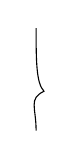
\begin{tikzpicture}\draw (0,0) .. controls (0,-.4) and (0,-.7) .. (.1,-.8)
.. controls (-.1,-.9) and (0,-1) .. (0,-1.3);\end{tikzpicture}}

\uline{NB} On trouve que la connexion respecte la filtration ssi
$\uline{c_{2,3}}=0$ (d'où $c_{1,2}=0$)
[ceci signifie: $\bar\omega_0=0$] ---
\deleted{\unsure{celles qui les}}
\inserted{ce sont aussi}
celles qui respectent le Borel $\mathcal L\subset\mathfrak g$,
i.e. encore celles qui respectent la section $\sigma$ de $P$, i.e. pour lesquelles
$\sigma$ est horizontale. Elles sont \unsure{différentiées|définies par}
une section de $\mathcal L\otimes\omega$.
\par \deleted{\unsure{Or $C$ est bien déterminé!, par des|Or $C$ est bien déterminé!, des}}

\margin{Re \uline{NB} On pourrait considérer
\diagram{\begin{tikzcd}
c^\Omega:\underset{\substack{\simeq\\\mathcal L^\vee\simeq\mathcal L\otimes\Omega^{-1}}}{\mathfrak g/\Omega}
\arrow[r]&\Omega^{-1}\otimes\uline\omega
\end{tikzcd}}
induit par $c$, \unsure{induisant $i$ (linéaire)|et devant être linéaire})
sur $\Omega^0\simeq O_X\subset\mathcal L\otimes\Omega^{-1}$.
Sa connaissance est \uline{équivalente} à celle de $C_\Omega$ si $2$ inv.,
et dans le cas général (p.e. en Car. $2$?) c'est \unsure{peut-être|encore} plus précis $\ldots$}
\figure{\begin{tikzpicture}[x=1cm,y=1cm]
\draw (0,2.3) .. controls (-.2,1.8) and (-.1,.4) .. (0,0)
.. controls (2,-.1) and (4,-.1) .. (6,-.3);
\draw[->] (-2,1) .. controls (-1.4,1.4) and (-.8,1.8) .. (-.5,2);
\end{tikzpicture}}

\uline{NB} Les connexions sur $\mathfrak g$ compatibles avec
crochet \deleted{\unsure{place|plat}}
(si $2$ inv. --- sinon il faut parler des connexions \inserted{\uline{Conn}}
sur $P$, ou $G$ etc) forment un torseur sous $\mathfrak g\otimes\uline\omega$. Or
\diagram{\begin{tikzcd}
{}\arrow[r,Rightarrow]&\mathfrak g\otimes\uline\omega\arrow[r]&\Omega^{-1}\otimes\uline\omega
\end{tikzcd}}
d'où un torseur sous $\Omega^{-1}\otimes\uline\omega$.
\uline{Ce dernier} est splitté canoniquement, i.e. on a
\diagram{\begin{tikzcd}
\uline{\mathrm{Conn}}\arrow[r,"\bar\omega_0"]&\Omega^{-1}\otimes\omega
\end{tikzcd}}
compatible avec $\unsure{\alpha|a}$, et si $c$ section de \uline{Conn},
$\bar\omega_0(c)$ détermine les hom
$\operatorname{gr}_i\mathfrak g\to\operatorname{gr}_{i+1}(\mathfrak g\otimes\uline\omega)$
\diagram{\begin{tikzcd}
\Omega=\operatorname{gr}_1(\mathfrak g)\arrow[r,"-2\bar\omega_0"']&
\omega\simeq\operatorname{gr}_2(\mathfrak g\otimes\unsure{\Omega|\omega})\\
\Omega^0\simeq O_X=\operatorname{gr}_2(\mathfrak g)\arrow[r,"\bar\omega_0"']&
\Omega^{-1}\otimes\uline\omega=\operatorname{gr}_3(\mathfrak g\otimes\uline\omega)
\end{tikzcd}}

Si on considère les $c$ pour lesquels
$\bar\omega_0(c)\in\underset{\substack{\Vert\\\operatorname{Hom}(\Omega,\uline\omega)}}{\Gamma\Omega^{-1}\otimes\uline\omega}$
est donné \inserted{$i$}, on donne une restriction
du Gr. struct. de \uline{Conn} à $\mathcal L\otimes\uline\omega$,
d'où torseur $\mathrm{Conn}_i$ sous $\mathcal L\otimes\uline\omega$. Or on a
\diagram{\begin{tikzcd}\mathcal L\otimes\uline\omega\arrow[r]&\uline\omega\end{tikzcd}}
d'où un torseur associé sous $\uline\omega$: les conn.
sur $\mathfrak g$ compatibles avec $i$, \uline{modulo} \inserted{\unsure{q.d.|i.e.}}
ajouter une section de $\Omega\otimes\uline\omega\subset\mathcal L\otimes\uline\omega\subset\mathfrak g\otimes\uline\omega$.
C'est aussi (\deleted{évidemment}) le torseur des restrictions
à $\Omega$ des conn. compatibles avec $i$, ou encore
des hom. additifs op. diff. d'ordre $1$ (rel. $S$
\diagram{\begin{tikzcd}\Omega\arrow[r,"C_\Omega"]&\mathcal L\otimes\omega\end{tikzcd}}
\unsure{telles|tels} que la composée
\diagram{\begin{tikzcd}
\deleted{\unsure{\mathcal L|\Omega}}\Omega\arrow[r,"C_\Omega"]&
\mathcal L\otimes\omega\arrow[r]&\omega
\end{tikzcd}}
soit linéaire (et égale à $-2i$), et que l'on ait
\[
C_\Omega(f\omega)-fC_\Omega(\omega)\simeq\omega\otimes df.
\qquad\begin{array}{l}\omega\in\Gamma\Omega\\f\in\Gamma O_X\end{array}
\]
\figure{\begin{tikzpicture}[x=1cm,y=1cm]
\draw (0,0)--(.05,.7)--(3.1,.7)--(3.3,0);
\draw (4,6)--(4.1,1);
\end{tikzpicture}}
\margin{verso}
\figure{\begin{tikzpicture}[x=1cm,y=1cm]
\draw (0,0)--(0,-.8);\draw (.07,.06)--(.07,-.7);
\draw (5,0)--(5,-.8);\draw (5.07,.06)--(5.07,-.7);
\end{tikzpicture}}

\scanpage{91}
% archive foliation: 90
La donnée d'un tel \deleted{(indép. de $i$)} $c_\Omega$ équivaut à une
\unsure{restriction|réduction} du Groupe structural de
$\uline{\mathrm{Conn}}_i\unsure{\xi|\varepsilon}$ à $\Omega\otimes\uline\omega$, ou encore
(indépendant de $i$) la donnée d'un $c_\Omega$ pour lequel
$(\unsure{A|*})$ est lin et $(**)$ est \unsure{vérif.|vérifié}, équivaut
à une restriction du Groupe structural
$\mathfrak g\otimes\omega$ de \uline{Conn} à $\Omega\otimes\uline\omega$.

On s'intéresse au cas où \deleted{\unsure{si|C}} $c_\Omega$ est
tel que la composée
\diagram{\begin{tikzcd}
(-2i):\Omega\arrow[r]&\mathcal L\otimes\uline\omega\arrow[r,dash]&\uline\omega
\end{tikzcd}}
\inserted{(\uline{ce qui implique $2$ inv.})}
soit un \uline{iso}. Alors le triplet
$(\mathfrak g,\mathcal L,c_\Omega)$
(\unsure{où|ou} ce qui revient au
$=$, $(\mathcal L\supset\Omega,c_\Omega)$) est défini à isom
unique près par $X/S$ (et existe ssi
$\uline\omega=\underline\Omega^1_{X/S}$ est inversible) comme
\[
\mathcal L\simeq P^1_{X/S}(\uline\omega)\otimes\uline\omega^{-1}
\qquad(\text{d'où }\mathcal L\otimes\uline\omega\simeq P^1_{X/S}(\uline\omega))
\]
et
\diagram{\begin{tikzcd}
c_\Omega:\Omega\simeq\uline\omega\arrow[r]&\mathcal L\otimes\uline\omega\simeq P^1_{X/S}(\uline\omega)
\end{tikzcd}}
n'est autre que
$d^1_{X/S,\underset{\uline\omega}{\unsure{\omega|\infty}}}$ --

\figure{\begin{tikzpicture}[x=1cm,y=1cm]
\draw (0,7)--(0,2.2) .. controls (0,.9) and (.2,.4) .. (1.4,-.1)
.. controls (2.4,-.5) and (2.9,-1.1) .. (4.5,-1.5);
\draw (2.1,4.4) .. controls (1.9,4.9) and (2.6,4.9) .. (3.4,4.9)
--(5.4,5.1);
\end{tikzpicture}}

